\documentclass[article]{jss}

%% -- LaTeX packages and custom commands ---------------------------------------

%% recommended packages
\usepackage{thumbpdf,lmodern,amsmath}

%% another package (only for this demo article)
\usepackage{framed}

%% new custom commands
\newcommand{\class}[1]{`\code{#1}'}
\newcommand{\fct}[1]{\code{#1()}}

%% For Sweave-based articles about R packages:
%% need no \usepackage{Sweave}



%% -- Article metainformation (author, title, ...) -----------------------------

%% - \author{} with primary affiliation
%% - \Plainauthor{} without affiliations
%% - Separate authors by \And or \AND (in \author) or by comma (in \Plainauthor).
%% - \AND starts a new line, \And does not.
\author{Hao Ye\\University of \\Florida
   \And Adam Clark\\German Centre for \\Integrative Biodiversity \\Research (iDiv)
   \And Ethan Deyle\\University of \\California San Diego
   \And George Sugihara\\University of \\California San Diego}
\Plainauthor{Hao Ye, Adam Clark, Ethan Deyle, George Sugihara}

%% - \title{} in title case
%% - \Plaintitle{} without LaTeX markup (if any)
%% - \Shorttitle{} with LaTeX markup (if any), used as running title
\title{\pkg{rEDM}: An \proglang{R} package for Empirical Dynamic Modeling and Convergent Cross Mapping}
\Plaintitle{rEDM: An R package for Empirical Dynamic Modeling and Convergent Cross Mapping}
\Shorttitle{\pkg{rEDM}: An \proglang{R} package for Empirical Dynamic Modeling}

%% - \Abstract{} almost as usual
\Abstract{
Empirical dynamic modeling (EDM) is an emerging non-parametric framework for modeling nonlinear dynamic systems. EDM is based on the mathematical theory of recontructing attractor manifolds from time series data \citep{Takens_1981}. The \pkg{rEDM} package collects several EDM methods, including simplex projection \citep{Sugihara_1990}, S-map \citep{Sugihara_1994}, multivariate embeddings \citep{Dixon_1999}, convergent cross mapping \citep{Sugihara_2012}, and multiview embedding \citep{Ye_2016}. Here, we introduce the basic underlying theory, and describe the functionality of \pkg{rEDM}, using examples from both model simulations and real data.
}

%% - \Keywords{} with LaTeX markup, at least one required
%% - \Plainkeywords{} without LaTeX markup (if necessary)
%% - Should be comma-separated and in sentence case.
\Keywords{time series, forecasting, causal inference, empirical dynamics, \proglang{R}}
\Plainkeywords{time series, forecasting, causal inference, empirical dynamics, R}

%% - \Address{} of at least one author
%% - May contain multiple affiliations for each author
%%   (in extra lines, separated by \emph{and}\\).
%% - May contain multiple authors for the same affiliation
%%   (in the same first line, separated by comma).
\Address{
  Hao Ye\\
  University of Florida\\
  Department of Wildlife Ecology and Conservation\\
  110 Newins-Ziegler Hall\\
  PO Box 110430\\
  Gainesville, FL 32611-0430\\
  E-mail: \email{hao.ye@weecology.org}%%\\
%%  URL: \url{https://eeecon.uibk.ac.at/~zeileis/}
}

\begin{document}


\section{Introduction} \label{sec:intro}

Many scientific fields use models as approximations of reality and for various purposes (e.g., testing hypotheses regarding mechanisms or processes, explaining past observations, predicting future outcomes). In most cases these models are based on hypothesized parametric equations; however explicit equations can be impractical when the exact mechanisms are unknown or too complex to be characterized with existing datasets. Empirical models, which infer patterns and associations from the data (instead of using hypothesized equations), represent an alternative and highly flexible approach. Here, we review the theoretical background for empirical dynamic modeling (EDM) and the functionality of the \pkg{rEDM} package, which are intended for nonlinear dynamic systems that can prove problematic for traditional modeling approaches.

The basic goal underlying EDM is to reconstruct the behavior of dynamic systems using time series data. This approach is based on mathematical theory developed initially by \citep{Takens_1981}, and subsequently expanded \citep{Sauer_1991, Casdagli_1991, Deyle_2011}. Because these methods operate with minimal assumptions, they are particularly suitable for studying systems that exhibit non-equilibrium dynamics and nonlinear state-dependent behavior (i.e., where interactions change over time and as a function of the system state).

\subsection{Installation}\label{sec:installation}

The \pkg{rEDM} package can be obtained in two main ways. The standard version of the package can be obtained through CRAN (the Comprehensive R Archive Network): \url{https://cran.r-project.org/package=rEDM}:

\begin{Schunk}
\begin{Sinput}
R> install.packages("rEDM")
\end{Sinput}
\end{Schunk}

However, the most recent version is available on GitHub: \url{https://github.com/ha0ye/rEDM}, and can be installed using the \code{install_github()} function in the \pkg{devtools} package.

\begin{Schunk}
\begin{Sinput}
R> devtools::install_github("ha0ye/rEDM")
\end{Sinput}
\end{Schunk}

\section{Empirical Dynamic Modeling}\label{sec:empirical-dynamic-modeling}

\subsection{Time Series as Observations of a Dynamic System}\label{sec:time-series}

The essential concept is that time series can be viewed as projections of the behavior of a dynamic system. Here, only a few modest assumptions are required. First, the system state can be described as a point in a high-dimensional space. The axes of this space can be thought of as fundamental state variables; in an ecosystem, these variables might correspond to population abundances, resources, or environmental conditions. Second, the system state changes through time following a set of deterministic rules. In other words, the behavior of the system is not completely stochastic.

Consequently, it is possible to project the system state onto one of the coordinate axes and obtain the value of the corresponding state variable. Sequential projections over time will thus produce a time series for that variable. For example, in Figure \ref{fig:time-series-projection}, the states of the canonical Lorenz Attractor \citep{Lorenz_1963} are projected to the $x$-axis, creating a time series of variable $x$.

\begin{figure}[t!]
\centering
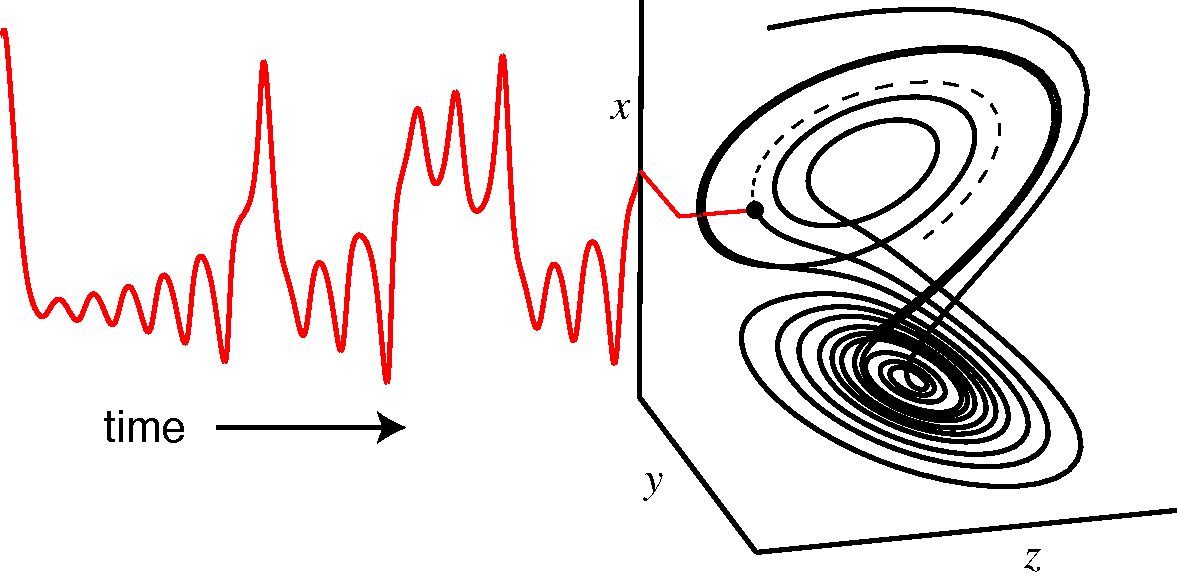
\includegraphics{figure_1}
\caption{\label{fig:time-series-projection} Time Series Projection from the Lorenz Attractor.}
\end{figure}

In simple cases, each time series will represent a different state variable. However, more generally, each time series is an \emph{observation function} of the system state, and may be a function of several different state variables. 

\subsection{Attractor Reconstruction / Takens' Theorem}\label{sec:attractor-reconstruction}

The goal of EDM is to reconstruct the system dynamics from time series data. Because time series are sequential observations of the system behavior, information about the rules that govern system behavior (i.e., the system dynamics) is therefore encoded in the data. Takens' Theorem \citep{Takens_1981} provides a way to recover this information using just a single time series. Although the system behavior is nominally determined by a high-dimensional state space, we can substitute lags of a time series for any unknown or unobserved variables. For example, instead of representing the system state of the Lorenz Attractor using $x$, $y$, and $z$, we can instead use an embedding that consists of \code{E} lags of $x$:
\begin{equation}
\mathbf{x}_t = \left( x_t, x_{t-\tau}, \dots, x_{t-(E-1)\tau} \right)
\end{equation}

\begin{figure}[t!]
\centering
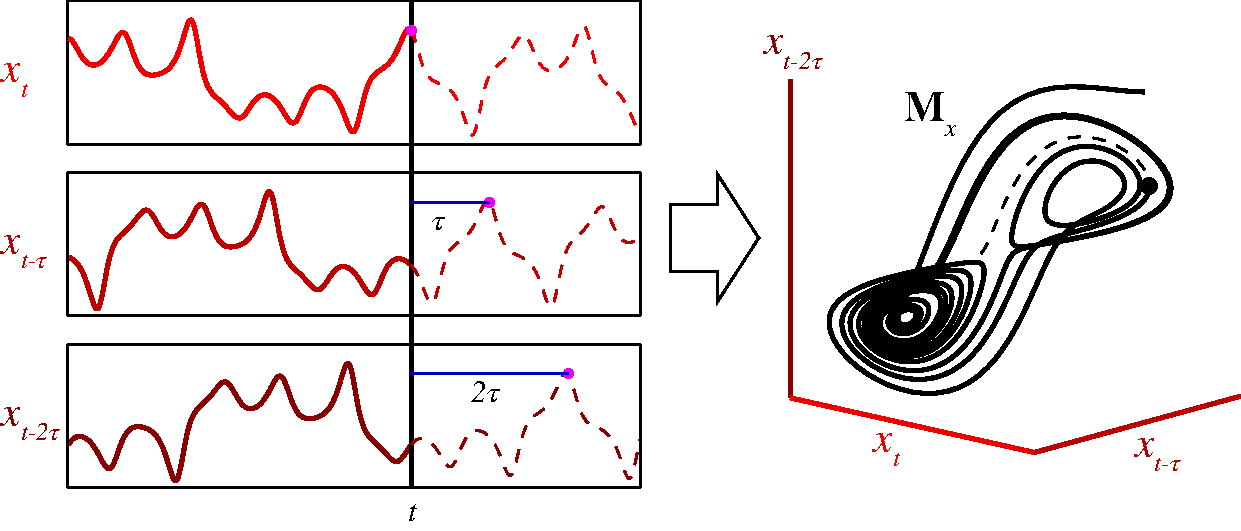
\includegraphics{figure_2}
\caption{\label{fig:attractor-reconstruction} Attractor Reconstruction using 3 Lagged Coordinates.}
\end{figure}

By Takens' Theorem, if sufficient lags are used, the reconstruction is a diffeomorphism of the original system. In other words, reconstructed states will map one-to-one to actual system states, and nearby points in the reconstruction will correspond to similar system states. Figure \ref{fig:attractor-reconstruction} shows a reconstruction of the Lorenz attractor where the reconstructed system state is comprised of 3 lags of variable $x$. There is a clear visual correspondence between the reconstruction and the original Lorenz attractor.

There are many applications for using this approach to recover system dynamics from time series. For example, empirical models can be used for forecasting \citep{Sugihara_1990}, to understand nonlinear behavior \citep{Sugihara_1994}, or to uncover mechanism \citep{Dixon_1999}. Recent work describes how EDM can be used to identify causal interactions, by testing whether two time series are observed from the same system \citep{Sugihara_2012}. In the next section, we demonstrate how the \pkg{rEDM} software package can be used to accomplish these tasks.

\section{EDM Examples}\label{sec:EDM-examples}

\subsection{Nearest Neighbor Forecasting using Simplex Projection}\label{sec:nearest-neighbor-forecasting}

As mentioned previously, if enough lags are used, the reconstruction will map one-to-one to the original attractor. However, if the number of lags is insufficient (i.e., the embedding dimension is too small), then the reconstruction will have singularities -- points that actually correspond to different system states, but which overlap in the reconstruction. When this occurs, the reconstruction will fail to distinguish between different trajectories, and forecast performance will suffer. Thus, prediction skill can be used as an indicator for the optimal embedding dimension.

In the following example, we demonstrate how to select the embedding dimension. We use a nearest neighbor forecasting method, Simplex Projection \citep{Sugihara_1990}, to produce forecasts, and examine prediction skill, computed as the correlation between observed and predicted values.

\subsubsection{Example}\label{sec:simplex-example}

In this example, time series come from a simulation of the tent map that exhibits chaotic behavior. The tent map is a discrete-time dynamic system, where a sequence, $x_t$, on the interval $[0, 1]$ is iterated according to:

\begin{equation*}
x_{t+1} =
\begin{cases}
2x_t, & x_t < \frac{1}{2}\\
2(1-x_t), & x_t \ge \frac{1}{2}
\end{cases}
\end{equation*}

In \pkg{rEDM}, a sample time series of the first-differenced values can be found in dataset \code{tentmap_del}.

We begin by loading the \pkg{rEDM} package:
\begin{Schunk}
\begin{Sinput}
R> library(rEDM)
\end{Sinput}
\end{Schunk}

Then, we can load the tentmap data:
\begin{Schunk}
\begin{Sinput}
R> data(tentmap_del)
R> str(tentmap_del)
\end{Sinput}
\begin{Soutput}
 num [1:999] -0.0992 -0.6013 0.7998 -0.7944 0.798 ...
\end{Soutput}
\end{Schunk}

We can see that the data consists of a single vector, containing the raw first-differences values of $x_t$. Because the \code{simplex()} function can accept a single vector as the input time series, no further processing of the data is required.

\begin{Schunk}
\begin{Sinput}
R> ts <- tentmap_del
R> lib <- c(1, 100)
R> pred <- c(201, 500)
\end{Sinput}
\end{Schunk}

We begin by initializing the \code{lib} and \code{pred} variables. These variables define the portions of the data that will be used to create the reconstruction. \code{lib} corresponds to the ``training'' portion of the data, on which nearest neighbors can be identified; and \code{pred} corresponds to the ``test'' portion of the data, on which 1-step ahead forecasts will be made. Here, the first 100 points (positions 1 to 100) in the time series constitute the ``library set'', and 300 points (positions 201 to 500) constitute the ``prediction set''.

The remaining arguments will be left at their default values (see section \ref{sec:general-parameters} for details). For the \code{simplex()} function, this means that the embedding dimension, \code{E}, will range from $1$ to $10$.

\emph{Note that if the code detects any overlap in the lib and pred, it will prevent a vector from becoming its own neighbor by enabling leave-one-out cross-validation and outputting a warning message.}

\begin{Schunk}
\begin{Sinput}
R> simplex_output <- simplex(ts, lib, pred)
R> str(simplex_output)
\end{Sinput}
\begin{Soutput}
'data.frame':	10 obs. of  16 variables:
 $ E                  : int  1 2 3 4 5 6 7 8 9 10
 $ tau                : num  1 1 1 1 1 1 1 1 1 1
 $ tp                 : num  1 1 1 1 1 1 1 1 1 1
 $ nn                 : num  2 3 4 5 6 7 8 9 10 11
 $ num_pred           : num  299 298 297 296 295 294 293 292 291 290
 $ rho                : num  0.847 0.962 0.942 0.91 0.874 ...
 $ mae                : num  0.207 0.102 0.138 0.19 0.235 ...
 $ rmse               : num  0.392 0.187 0.236 0.291 0.334 ...
 $ perc               : num  0.853 0.906 0.899 0.885 0.824 ...
 $ p_val              : num  2.59e-102 4.99e-253 4.65e-199 1.54e-151 2.59..
 $ const_pred_num_pred: num  299 298 297 296 295 294 293 292 291 290
 $ const_pred_rho     : num  -0.668 -0.671 -0.671 -0.673 -0.671 ...
 $ const_pred_mae     : num  1.02 1.02 1.02 1.02 1.01 ...
 $ const_pred_rmse    : num  1.25 1.25 1.26 1.26 1.25 ...
 $ const_pred_perc    : num  0.341 0.339 0.337 0.338 0.339 ...
 $ const_p_val        : num  1 1 1 1 1 1 1 1 1 1
\end{Soutput}
\end{Schunk}

The output is a data.frame with columns for each of the model parameters and forecast statistics, and rows for each separate model (i.e., different parameter combinations). For Simplex Projection, the model parameters are \code{E}, embedding dimension; \code{tau}, time lag between successive dimensions; \code{tp}, time to prediction; and \code{nn}, number of nearest neighbors. The forecast statistics are \code{num_pred}, the number of predictions made; \code{rho}, Pearson's correlation coefficient between predictions and observations; \code{mae}, mean absolute error of predictions; \code{rmse}, root mean squared error of predictions; \code{perc}, the percent of predictions that are the same sign as observations; and \code{p_val}, the p-value for \code{rho} being significantly greater than 0, using Fisher's transformation \citep{Fisher_1915}. For the purpose of comparison, the last 6 columns give those same forecast statistics, but for a naive constant predictor (where the 1-step ahead forecast is the current value) over the same set of predictions.

In this case, there are 10 separate models (one for each value of \code{E}), so we can plot \code{E} against \code{rho} (the correlation between observed and predicted values) to determine the optimal embedding dimension (i.e., the number of dimensions for which the reconstructed attractor is best unfolded, producing the highest forecast skill).

\begin{Schunk}
\begin{Sinput}
R> par(mar = c(4, 4, 1, 1), mgp = c(2.5, 1, 0))
R> plot(simplex_output$E, simplex_output$rho, type = "l",  
+       xlab = "Embedding Dimension (E)", ylab = "Forecast Skill (rho)")
\end{Sinput}
\end{Schunk}

\begin{figure}[t!]
\centering
\includegraphics[width=4.5in]{article-simplex-e}
\caption{\label{fig:simplex-e} \code{rho} vs. \code{E} for the tent map.}
\end{figure}

In Figure \ref{fig:simplex-e}, we observe that forecast skill peaks at \code{E = 2}, indicating that the dynamics of our data are unfolded best in 2 dimensions. \emph{Note that this optimal value does not have to correspond to the dimensionality of the original system.}  The forecast skill will be affected by factors such as observational noise, process error, and time series length, and so it is more useful to think of the embedding dimension as a practical measure that is dependent on properties of the data.

\subsection{Prediction Decay}\label{sec:prediction-decay}

An important property of many natural systems is that nearby trajectories eventually diverge over time (i.e., ``deterministic chaos'' -- the ``butterfly effect''). In essence, this means that while short-term prediction is often possible, information about the state of the system is continually lost over time, hindering long-term prediction. We can demonstrate this effect by examining how prediction skill changes as we increase the \code{tp} argument, the ``time to prediction'', the number of time steps into the future that forecasts are made.

\subsubsection{Example}\label{sec:prediction-decay-example}

Using the same data and the \code{simplex()} function, we supply a range for the \code{tp} argument and fix the embedding dimension to the value determined previously (\code{E = 2}):

\begin{Schunk}
\begin{Sinput}
R> simplex_output <- simplex(ts, lib, pred, E = 2, tp = 1:10)
\end{Sinput}
\end{Schunk}

As above, the returned object is a data.frame, so we can examine prediction decay by plotting forecast skill (\code{rho}) against the time to prediction (\code{tp}):

\begin{Schunk}
\begin{Sinput}
R> par(mar = c(4, 4, 1, 1), mgp = c(2.5, 1, 0))
R> plot(simplex_output$tp, simplex_output$rho, type = "l",
+       xlab = "Time to Prediction (tp)", ylab = "Forecast Skill (rho)")
\end{Sinput}
\end{Schunk}

\begin{figure}[t!]
\centering
\includegraphics[width=4.5in]{article-simplex-tp}
\caption{\label{fig:simplex-tp} \code{rho} vs. \code{tp} for the tent map.}
\end{figure}

Because the parameters for the tent map fall in the region for chaotic behavior, there is a noticeable decline in forecast skill as \code{tp} increases (Figure \ref{fig:simplex-tp}).

\subsection{Identifying Nonlinearity}\label{sec:nonlinearity}

One concern is that time series may show predictability even if they are purely stochastic, because they have temporal autocorrelation (i.e., similar to autocorrelated red noise). We can distinguish between red noise and nonlinear deterministic behavior by using S-maps as described in \citet{Sugihara_1994}.

In contrast to the nearest-neighbor interpolation of simplex projection, the S-map forecasting method \citep{Sugihara_1994} fits local linear maps to forecast from the reconstructed state space. Here, ``local'' means that the map can be different at different locations in the reconstructed state space.

With S-maps, the nonlinear tuning parameter, $\theta$, determines the strength of the weighting when fitting the lcoal linear map. For example, when $\theta = 0$, all points always receive equal weighting. In other words, the local linear map does not change, and will be identical to a global linear map -- equivalent to fitting an autoregressive model to the data. In contrast, when $\theta > 0$, nearby points receive larger weights, allowing the local linear map to vary in state-space and accommodate nonlinear behavior (see the ``rEDM-algorithms'' vignette for more details).

Consequently, if the time series are sampled from autoregressive red noise, then there will be no improvement to forecast skill when $\theta > 0$. In fact, it is likely that the linear model ($\theta = 0$) produces the best forecasts, because it uses all the data for constructing the global linear map, thereby reducing the effects of observational noise. Thus, increases in forecast skill when $\theta > 0$ is indicative of nonlinear dynamics; allowing the local linear map to vary in state-space produces a better description of state-dependent behavior.

\subsubsection{Example}\label{nonlinearity-example}

The S-map method is implemented as the function \code{s_map()} in the \pkg{rEDM} package. Following from the previous example, we again use the tent map time series, and set \code{E = 2} based on the results from simplex projection. Note that we allow many of the arguments to take on default values (e.g., \code{tau = 1}, \code{tp = 1}). If we had changed these for simplex projection, we would want to propagate them here. The default values for the nonlinear tuning parameter, \code{theta}, range from \code{0} to \code{8}, and are suitable for our purposes.

Note also, that the default value for \code{num_neighbors} is \code{0}. When using S-maps to test for nonlinear behavior, we want to use all points in the reconstruction, and allow \code{theta} to control the weighting assigned to individual points. By using \code{0} for this argument (an otherwise nonsensical value), the program will use all nearest neighbors.

\begin{Schunk}
\begin{Sinput}
R> smap_output <- s_map(ts, lib, pred, E = 2)
\end{Sinput}
\end{Schunk}

Again, the results are a data.frame with columns for each of the model parameters and forecast statistics, with rows for each run of the model. In this case, there is one run for each value of \code{theta}, so we can simply plot \code{theta} against \code{rho}:

\begin{Schunk}
\begin{Sinput}
R> par(mar = c(4, 4, 1, 1), mgp = c(2.5, 1, 0))
R> plot(smap_output$theta, smap_output$rho, type = "l",
+       xlab = "Nonlinearity (theta)", ylab = "Forecast Skill (rho)")
\end{Sinput}
\end{Schunk}

\begin{figure}[t!]
\centering
\includegraphics[width=4.5in]{article-smap-theta}
\caption{\label{fig:smap-theta} \code{rho} vs. \code{theta} for the tent map.}
\end{figure}

Here, we can see that forecast skill substantially improves as \code{theta} increases, indicating the presence of nonlinear dynamics (Figure \ref{fig:smap-theta}). Typically, we would expect forecast skill to begin to decrease at high values of \code{theta}, because the local linear map will overfit to the nearest points. However, because the example data are observed without any noise, we continue to get a better approximation to the true function with higher \code{theta}.

\begin{Schunk}
\begin{Sinput}
R> par(mar = c(4, 4, 1, 1), mgp = c(2.5, 1, 0))
R> ts_err <- ts + rnorm(length(ts), sd = sd(ts) * 0.2)
R> smap_output_err <- s_map(ts_err, lib, pred, E = 2)
R> plot(smap_output_err$theta, smap_output_err$rho, type = "l",
+       xlab = "Nonlinearity (theta)", ylab = "Forecast Skill (rho)")
\end{Sinput}
\end{Schunk}

\begin{figure}[t!]
\centering
\includegraphics[width=4.5in]{article-smap-theta-noisy}
\caption{\label{fig:smap-theta-noisy} \code{rho} vs. \code{theta} for the tent map (with simulated noise).}
\end{figure}

By simulating the addition of a small amount of observational noise, a plot more typical of real data can be achieved (Figure \ref{fig:smap-theta-noisy}).

\subsection{Generalized Takens' Theorem}\label{sec:generalized-takens-theorem}

In addition to creating an attractor from lags of one time series, it is possible to combine different time series, if they are all observed from the same system \citep{Sauer_1991, Deyle_2011}. The practical reality of complex dynamics, finite, noisy data, and stochastic drivers means that ``multivariate'' reconstructions can often be a better description than ``univariate'' reconstructions.

In \pkg{rEDM}, the \code{block_lnlp()} function generalizes the \code{simplex()} and \code{s_map()} functions: reconstructions can be formed from any set of coordinates, and forecasts are made using either of the two methods.

The data format for \code{block_lnlp()} is a matrix or data.frame, where each column is a separate time series, and each row is a temporal ``slice'' of the data comprised of simultaneous observations. A reconstruction is defined by specifying which columns to use as coordinates (the \code{columns} argument) and which column is to be forecast (the \code{target_column} argument). If lagged copies of a time series are desired as coordinates, they need to be pre-computed as separate columns in the input (e.g., via the \code{make_block()} function).

\subsubsection{Example}\label{sec:block-lnlp-example}

We begin by loading an example dataset from a coupled 3-species model system.

\begin{Schunk}
\begin{Sinput}
R> data(block_3sp)
R> str(block_3sp)
\end{Sinput}
\begin{Soutput}
'data.frame':	200 obs. of  10 variables:
 $ time : int  1 2 3 4 5 6 7 8 9 10 ...
 $ x_t  : num  -0.742 1.245 -1.918 -0.962 1.332 ...
 $ x_t-1: num  NA -0.742 1.245 -1.918 -0.962 ...
 $ x_t-2: num  NA NA -0.742 1.245 -1.918 ...
 $ y_t  : num  -1.268 1.489 -0.113 -1.107 2.385 ...
 $ y_t-1: num  NA -1.268 1.489 -0.113 -1.107 ...
 $ y_t-2: num  NA NA -1.268 1.489 -0.113 ...
 $ z_t  : num  -1.864 -0.482 1.535 -1.493 -1.119 ...
 $ z_t-1: num  NA -1.864 -0.482 1.535 -1.493 ...
 $ z_t-2: num  NA NA -1.864 -0.482 1.535 ...
\end{Soutput}
\end{Schunk}

Here, the \code{block_3sp} variable is a 10-column data.frame with 1 column for time, and 3 columns for each of the variables (unlagged: $t$, lag-1: $t-1$, and lag-2: $t-2$). Note that the lagged columns begin with \code{NA} values because there are no observations of the variables for times $t < 1$. The vectors that include \code{NA} values are excluded if that specific value is needed for computation (see section \ref{sec:data-input} for more details).

Columns can be referred to using either numerical indices or the column names. If numerical indices are used, \code{block_lnlp} has an option to indicate that the first column is actually a time index. When \code{first_column_time} is set to \code{TRUE}, a value of \code{1} for \code{target_column} will point to the first \emph{data} column in the data.frame.

\begin{Schunk}
\begin{Sinput}
R> lib <- c(1, NROW(block_3sp))
R> pred <- c(1, NROW(block_3sp))
R> cols <- c(1, 2, 4)
R> target <- 1
R> output <- block_lnlp(block_3sp, lib = lib, pred = pred,
+                       columns = cols, target_column = target,
+                       stats_only = FALSE, first_column_time = TRUE, 
+                       silent = TRUE)
\end{Sinput}
\end{Schunk}

We can also refer to columns by the column names. This ignores the \code{first_column_time} argument when referring to columns, but does use the time column to label predictions:

\begin{Schunk}
\begin{Sinput}
R> output_2 <- block_lnlp(block_3sp, lib = lib, pred = pred,
+                         columns = c("x_t", "x_t-1", "y_t"), 
+                         target_column = "x_t",
+                         stats_only = FALSE, first_column_time = TRUE, 
+                         silent = TRUE)
R> # test for equality
R> stopifnot(identical(output, output_2))
\end{Sinput}
\end{Schunk}

Note that the default value for the \code{tp} argument is \code{1}, indicating that predictions are 1-step ahead (i.e., using each row of the \code{columns} variables to predict the subsequent row of the \code{target_column} variable). \emph{In some cases, the data may be formatted to have the predicted variable aligned in the same row (but in a different column), and \code{tp} should be set to \code{0}.}

\begin{Schunk}
\begin{Sinput}
R> str(output)
\end{Sinput}
\begin{Soutput}
'data.frame':	1 obs. of  16 variables:
 $ embedding          : chr "1, 2, 4"
 $ tp                 : num 1
 $ nn                 : num 4
 $ num_pred           : num 198
 $ rho                : num 0.875
 $ mae                : num 0.32
 $ rmse               : num 0.43
 $ perc               : num 0.889
 $ p_val              : num 6.83e-80
 $ const_pred_num_pred: num 198
 $ const_pred_rho     : num -0.539
 $ const_pred_mae     : num 1.31
 $ const_pred_rmse    : num 1.55
 $ const_pred_perc    : num 0.394
 $ const_p_val        : num 1
 $ model_output       :List of 1
  ..$ :'data.frame':	200 obs. of  4 variables:
  .. ..$ time    : num  2 3 4 5 6 7 8 9 10 11 ...
  .. ..$ obs     : num  1.245 -1.918 -0.962 1.332 -0.817 ...
  .. ..$ pred    : num  NaN -1.226 -0.657 0.872 -1.59 ...
  .. ..$ pred_var: num  NaN 0.328 0.522 0.236 0.244 ...
  ..- attr(*, "class")= chr "AsIs"
\end{Soutput}
\end{Schunk}

By setting \code{stats_only} to \code{FALSE}, the output also includes the observed and predicted values in a list column (\code{model_output}). Unlike other columns, which are vectors of simple types (e.g., numeric, character), the \code{model_output} column is a list of length 1, whose single element is a data.frame of the observed and predicted values. If we had run multiple models, the \code{model_output} column would be a list of multiple data.frames (one data.frame of observed and predicted values for each model).

To compare the observed and predicted values, we want to pull out the appropriate columns:
\begin{Schunk}
\begin{Sinput}
R> list_of_model_predictions <- output$model_output
R> first_data_frame_of_predictions <- list_of_model_predictions[[1]]
R> observed <- first_data_frame_of_predictions$obs
R> predicted <- first_data_frame_of_predictions$pred
\end{Sinput}
\end{Schunk}

We can compare predicted vs. observed in a square plot with a 1:1 line (Figure \ref{fig:block-lnlp-obs-vs-pred}):

\begin{Schunk}
\begin{Sinput}
R> par(pty = "s", mar = c(4, 4, 1, 1), mgp = c(2.5, 1, 0))
R> plot_range <- range(c(observed, predicted), na.rm = TRUE)
R> plot(observed, predicted, xlim = plot_range, ylim = plot_range,
+       xlab = "Observed", ylab = "Predicted", asp = 1)
R> abline(a = 0, b = 1, lty = 2, col = "blue")
\end{Sinput}
\end{Schunk}

\begin{figure}[t!]
\centering
\includegraphics[width=3.5in]{article-block-lnlp-obs-vs-pred}
\caption{\label{fig:block-lnlp-obs-vs-pred} Predicted vs. Observed for a multivariate model of a coupled 3-species system.}
\end{figure}

\subsection{S-map Coefficients}\label{sec:s-map-coefficients}

As described in \citet{Deyle_2016}, the S-map coefficients from the appropriate multivariate embedding can be interpreted as dynamic, time-varying interaction strengths. We demonstrate this approach for the same 3-species simulation as above, using \code{x}, \code{y}, and \code{z} as the coordinates to predict \code{x}.

\begin{Schunk}
\begin{Sinput}
R> data(block_3sp)
R> lib <- c(1, 100)
R> pred <- c(101, 200)
R> cols <- c("x_t", "y_t", "z_t")
R> target <- "x_t"
R> output <- block_lnlp(block_3sp, lib = lib, pred = pred,
+                       columns = cols, target_column = target, 
+                       method = "s-map", theta = 2, 
+                       stats_only = FALSE, first_column_time = TRUE, 
+                       save_smap_coefficients = TRUE, silent = TRUE)
\end{Sinput}
\end{Schunk}

\begin{figure}[t!]
\centering
\includegraphics[width=5in]{article-smap-coefficients}
\caption{\label{fig:smap-coefficients} Time series and S-map coefficients for a multivariate model of a coupled 3-species system.}
\end{figure}

The \code{smap_coefficients} column of the output is a list-column with the data.frames for the S-map coefficients of each model. Since we have just have one model, we just want the first element of that list. The result is a data.frame with 200 rows (for each prediction) and 4 columns (for each of the 3 predictors and a constant).

\begin{Schunk}
\begin{Sinput}
R> smap_coeffs <- output$smap_coefficients[[1]]
R> str(smap_coeffs)
\end{Sinput}
\begin{Soutput}
'data.frame':	100 obs. of  4 variables:
 $ c_1: num  -1.561 0.394 -1.112 -0.801 -1.487 ...
 $ c_2: num  -0.2263 0.0216 -0.164 0.0315 -0.1408 ...
 $ c_3: num  -0.34154 0.12711 -0.22768 0.03366 0.00995 ...
 $ c_0: num  0.63 0.668 0.397 0.388 0.555 ...
\end{Soutput}
\end{Schunk}

Here, we plot the time series for the observed (solid) and predicted (dashed) values of \code{x} in the top panel; and the inferred interactions (s-map coefficients) for the influence of \code{x}, \code{y}, and \code{z} on future values of \code{x} in the remaining 3 panels (Figure \ref{fig:smap-coefficients}).

\begin{Schunk}
\begin{Sinput}
R> par(mfrow = c(4, 1), mar = c(2, 4, 1, 1), mgp = c(2.5, 1, 0))
R> predictions <- output$model_output[[1]]
R> t <- predictions$time
R> plot(t, predictions$obs, type = "l", col = "black", ylab = "x", xlab = "")
R> lines(t, predictions$pred, lty = 2)
R> legend("topright", legend = c("observed", "predicted"), lty = c(1, 2), 
+         bg = "white")
R> plot(t, smap_coeffs[, 1], type = "l", col = "red", 
+       ylab = "effect of x", xlab = "")
R> plot(t, smap_coeffs[, 2], type = "l", col = "blue", 
+       ylab = "effect of y", xlab = "")
R> plot(t, smap_coeffs[, 3], type = "l", col = "magenta", 
+       ylab = "effect of z", xlab = "")
\end{Sinput}
\end{Schunk}

\subsection{Gaussian Process}\label{sec:gaussian-processes}

An alternative approach to using Simplex Projection or S-maps is to use Gaussian Processes (GP). In the \pkg{rEDM} package, the equivalent function to the univariate \code{simplex()} and \code{s_map()} is \code{tde_gp()} (for ``Time Delay Embedding using Gaussian Processes'') and the equivalent function to the general \code{block_lnlp()} is \code{block_gp()}.

Note that the arguments are slightly different: the GP formulation includes hyperparameters for fitting to the data (\code{phi}, \code{v_e}, and \code{eta}). These can be set directly, or fit over the points in the \code{lib} portion of the data. In addition, the GP specifies not only pointwise error estimates for the predicted points, but also the covariance between them. In other words, the uncertainty for nearby points, in the state-space of the reconstructed attractor, is correlated. Setting \code{save_covariance_matrix = TRUE} will also return the full covariance matrix for the predicted points in the output of these functions. For more details, please see the documentation for \code{tde_gp()} and \code{block_gp()}.

We repeat the above example, but using \code{block_gp()} instead of \code{block_lnlp()}. 

\begin{Schunk}
\begin{Sinput}
R> data(block_3sp)
R> lib <- c(1, NROW(block_3sp))
R> pred <- c(1, NROW(block_3sp))
R> cols <- c(1, 2, 4)
R> target <- 1
R> output <- block_gp(block_3sp, lib = lib, pred = pred,
+                     columns = cols, target_column = target,
+                     stats_only = FALSE, first_column_time = TRUE, 
+                     silent = TRUE)
R> str(output)
\end{Sinput}
\begin{Soutput}
'data.frame':	1 obs. of  13 variables:
 $ embedding   : Factor w/ 1 level "1, 2, 4": 1
 $ tp          : num 1
 $ phi         : num 0.289
 $ v_e         : num -2.03
 $ eta         : num 2.01
 $ fit_params  : logi TRUE
 $ num_pred    : num 198
 $ rho         : num 0.949
 $ mae         : num 0.214
 $ rmse        : num 0.281
 $ perc        : num 0.924
 $ p_val       : num 2.15e-142
 $ model_output:List of 1
  ..$ :'data.frame':	198 obs. of  4 variables:
  .. ..$ time    : num  3 4 5 6 7 8 9 10 11 12 ...
  .. ..$ obs     : num  -1.918 -0.962 1.332 -0.817 0.744 ...
  .. ..$ pred    : num  -1.376 -0.888 1.063 -1.097 0.959 ...
  .. ..$ pred_var: num  0.114 0.112 0.128 0.147 0.107 ...
\end{Soutput}
\end{Schunk}

The output is nearly identical to that of \code{block_lnlp()}, but with slightly different columns - the GP hyperparameters are included instead of the number of neighbors and \code{theta} parameters.

To compare the observed and predicted values, we can again use the data.frame from the \code{model_output} column (Figure \ref{fig:gp-obs-vs-pred}):

\begin{Schunk}
\begin{Sinput}
R> observed <- output$model_output[[1]]$obs
R> predicted <- output$model_output[[1]]$pred
R> par(pty = "s", mar = c(4, 4, 1, 1), mgp = c(2.5, 1, 0))
R> plot_range <- range(c(observed, predicted), na.rm = TRUE)
R> plot(observed, predicted, xlim = plot_range, ylim = plot_range,
+       xlab = "Observed", ylab = "Predicted", asp = 1)
R> abline(a = 0, b = 1, lty = 2, col = "blue")
\end{Sinput}
\end{Schunk}

\begin{figure}[t!]
\centering
\includegraphics[width=3.5in]{article-gp-obs-vs-pred}
\caption{\label{fig:gp-obs-vs-pred} Predicted vs. Observed for a Gaussian Process model of a coupled 3-species system.}
\end{figure}

\subsection{Multiview Embedding}\label{sec:multiview-embedding}

The generality of Takens' Theorem means that in situations with multivariate time series, there can often be many different, valid attractor reconstructions. As described in \citet{Ye_2016}, combining these different models can result in improved forecasts.

Here, we demonstrate this idea using the \code{multiview()} function and with the same dataset as above. \code{multiview()} operates by constructing all possible embeddings of dimension \code{E}, with lag up to \code{max_lag} (and excluding embeddings that don't have at least one coordinate with 0 time lag). These embeddings are ranked by forecast skill (\code{rho}) over the \code{lib} portion of the data. The individual forecasts for the top \code{k} embeddings are then averaged together.

\begin{Schunk}
\begin{Sinput}
R> data("block_3sp")
R> block <- block_3sp[, c(2, 5, 8)] # use only the unlagged time series
R> lib <- c(1, floor(NROW(block_3sp) / 2))
R> pred <- c(floor(NROW(block_3sp) / 2) + 1, NROW(block_3sp))
R> # multiple values for \code{k} can be provided, 
R> #   "sqrt" uses floor(sqrt(m)), where m is the number of embeddings
R> k_list <- c(1, 3, "sqrt", "all")
R> output <- multiview(block, lib = lib, pred = pred,
+                      E = 3, max_lag = 3, target_column = 1, 
+                      k = k_list, stats_only = FALSE, 
+                      save_lagged_block = TRUE, silent = TRUE)
R> str(output, max.level = 1)
\end{Sinput}
\begin{Soutput}
'data.frame':	4 obs. of  14 variables:
 $ E           : num  3 3 3 3
 $ tau         : num  1 1 1 1
 $ tp          : num  1 1 1 1
 $ nn          : num  4 4 4 4
 $ k           : num  1 3 8 64
 $ num_pred    : num  99 99 99 99
 $ rho         : num  0.846 0.902 0.908 0.851
 $ mae         : num  0.351 0.272 0.259 0.373
 $ rmse        : num  0.459 0.354 0.34 0.469
 $ perc        : num  0.848 0.899 0.939 0.919
 $ p_val       : num  2.00e-34 2.96e-48 2.26e-50 3.12e-35
 $ model_output:List of 4
  ..- attr(*, "class")= chr "AsIs"
 $ lagged_block:List of 4
  ..- attr(*, "class")= chr "AsIs"
 $ embeddings  :List of 4
\end{Soutput}
\end{Schunk}

Note that the output has information about 3 models, since we specified 3 different values for \code{k}. Here, \code{lagged_block} gives the block that includes lags constructed for multiview embedding, and \code{embeddings} gives the list of the embeddings that were averaged together for each model.

Again, we can compare the observed and predicted values using the data.frame from the \code{model_output} column:

\begin{Schunk}
\begin{Sinput}
R> par(pty = "s", mfrow = c(2, 2), 
+      mar = c(4, 4, 1, 1), mgp = c(2.5, 1, 0))
R> for (i in 1:4)
+  {
+      preds <- output$model_output[[i]]
+      
+      plot_range <- range(c(preds$obs, preds$pred), na.rm = TRUE)
+      plot(preds$obs, preds$pred, 
+           xlim = plot_range, ylim = plot_range,
+           xlab = "Observed", ylab = "Predicted", asp = 1, 
+           main = paste0(output$k[i], " embeddings"))
+      abline(a = 0, b = 1, lty = 2, col = "blue")
+  }
\end{Sinput}
\end{Schunk}

\begin{figure}[t!]
\centering
\includegraphics[width=6in]{article-multiview}
\caption{\label{fig:multiview} Predicted vs. Observed for Multiview Embeddings of a coupled 3-species system.}
\end{figure}

\subsection{Causal Inference and Cross Mapping}\label{sec:causality}

One of the corollaries to Takens' Theorem is that multiple reconstructions not only map to the original system, but also to each other. Consider two variables, $x$ and $y$ that interact in a dynamic system. The univariate reconstructions based on lags of $x$ ($\mathbf{M}_x$) or $y$ ($\mathbf{M}_y$) are each capable of uniquely identifying system states. Thus, the reconstructed states of $\mathbf{M}_x$ map to reconstructed states of $\mathbf{M}_y$. This suggests a way to test whether $x$ and $y$ interact in the same system, by testing for a mapping between $\mathbf{M}_x$ and $\mathbf{M}_y$. Practically this is done by testing the predictive skill for the mapping from $\mathbf{M}_x$ to $y$ and from $\mathbf{M}_y$ to $x$.

\begin{figure}[t!]
\begin{center}
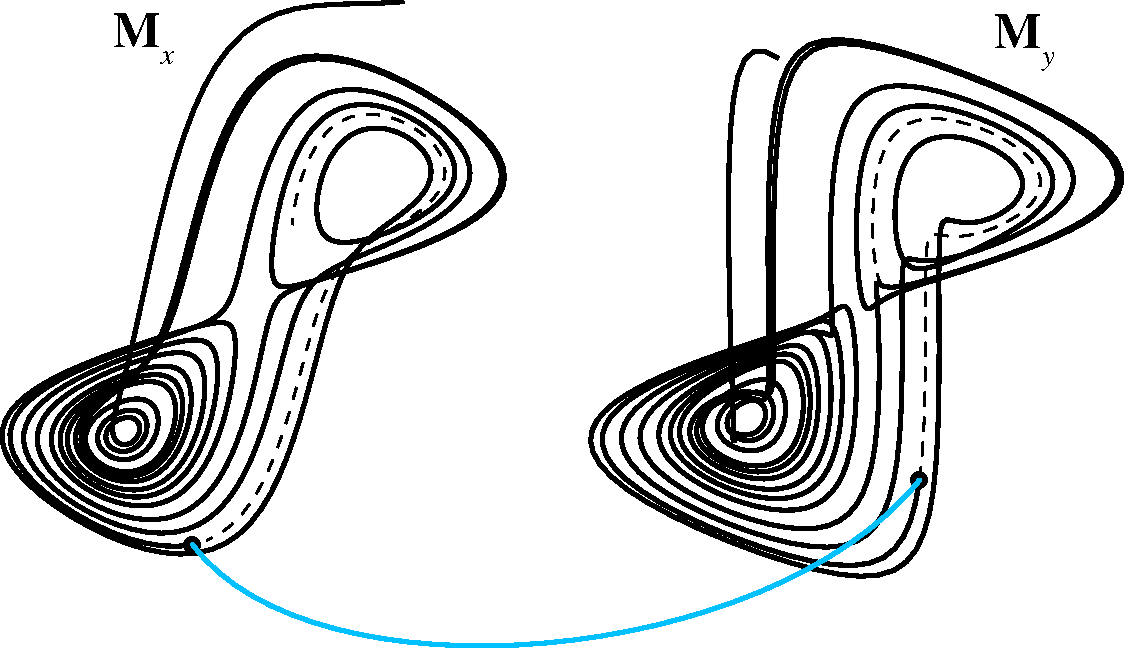
\includegraphics{figure_3}
\end{center}
\caption{\label{fig:cross-mapping} Cross Mapping Between Reconstructions of the Lorenz Attractor.}
\end{figure}

Furthermore, in the case of unidirectional causality, e.g., $x$ causes $y$, but $y$ does not cause $x$, we would only expect cross mapping to be successful in one direction. Somewhat counterintuitively, if a causal variable ($x$) leaves a signature on the affected variable ($y$), then it is possible to map from $\mathbf{M}_y$ to $\mathbf{M}_x$, but not vice-versa.

In essence, $\mathbf{M}_y$ must have complete information about $y$, which means it must include information about all its causes, including $x$. However, because $x$ behaves independently of $y$, the reconstruction $\mathbf{M}_x$ may be missing information about $y$, preventing a \emph{complete} cross mapping from $\mathbf{M}_x$ to $y$.

To be more precise, although $x$ has incomplete information about $y$, it does have a causal influence on $y$, and there will likely be some predictive skill in the mapping from $\mathbf{M}_x$ to $y$. However, this will be limited to the statistical association between $x$ and $y$ and will generally not improve with more data.

In contrast, the mapping from $\mathbf{M}_y$ to $x$ is expected to become complete with more data. This convergence is a critical property for inferring causality, and can be tested by measuring the cross mapping skill when using different amounts of data to reconstruct $\mathbf{M}_y$. For a more detailed description of using cross mapping to infer causation, see \citet{Sugihara_2012, Ye_2015a}.

\subsection{Convergent Cross Mapping (CCM)}\label{sec:ccm}

In \pkg{rEDM}, convergent cross mapping is implemented as the \code{ccm()} function, which provides a wrapper to compute cross map skill for different subsamples of the data. In the following example, we reproduce the analysis from \citet{Sugihara_2012} to identify causality between anchovy landings in California and Newport Pier sea-surface temperature. For this example, we use the previously identified embedding dimension of \code{E = 3}.

To identify convergence, we compute cross-map skill (Pearson's correlation, $\rho$ between observed and predicted values) over many random subsamples of the time series. The \code{lib_sizes} argument specifies the size of the library set, and \code{num_samples} specifies the number of subsamples generated at each library size. \code{random_libs} and \code{replace} specify how the subsamples will be generated. Here, setting both to \code{TRUE} enables random sampling with replacement.

\begin{Schunk}
\begin{Sinput}
R> data(sardine_anchovy_sst)
R> anch_xmap_sst <- ccm(sardine_anchovy_sst, E = 3,
+                       lib_column = "anchovy", target_column = "np_sst",
+                       lib_sizes = seq(10, 80, by = 10), num_samples = 100,
+                       random_libs = TRUE, replace = TRUE, silent = TRUE)
R> sst_xmap_anch <- ccm(sardine_anchovy_sst, E = 3,
+                       lib_column = "np_sst", target_column = "anchovy",
+                       lib_sizes = seq(10, 80, by = 10), num_samples = 100,
+                       random_libs = TRUE, replace = TRUE, silent = TRUE)
R> str(anch_xmap_sst)
\end{Sinput}
\begin{Soutput}
'data.frame':	800 obs. of  11 variables:
 $ E            : num  3 3 3 3 3 3 3 3 3 3 ...
 $ tau          : num  1 1 1 1 1 1 1 1 1 1 ...
 $ tp           : num  0 0 0 0 0 0 0 0 0 0 ...
 $ nn           : num  4 4 4 4 4 4 4 4 4 4 ...
 $ lib_column   : Factor w/ 1 level "anchovy": 1 1 1 1 1 1 1 1 1 1 ...
 $ target_column: Factor w/ 1 level "np_sst": 1 1 1 1 1 1 1 1 1 1 ...
 $ lib_size     : num  10 10 10 10 10 10 10 10 10 10 ...
 $ num_pred     : num  76 76 76 76 76 76 76 76 76 76 ...
 $ rho          : num  -0.18294 -0.00919 0.0888 0.15243 0.12651 ...
 $ mae          : num  0.967 1.174 0.912 0.83 0.923 ...
 $ rmse         : num  1.17 1.42 1.12 1.06 1.17 ...
\end{Soutput}
\end{Schunk}

The output is a data.frame with statistics for each model run (in this case, 100 models at each of 8 library sizes). To interpret the results, we aggregate the cross map performance at each library size using the \code{ccm_means()} function, which computes a mean value at each unique \code{lib_size}. Because average cross map skill less than 0 means there is no prediction skill, (predictions should not be anticorrelated with observations), we set negative values to 0 when plotting.

\begin{Schunk}
\begin{Sinput}
R> a_xmap_t_means <- ccm_means(anch_xmap_sst)
R> t_xmap_a_means <- ccm_means(sst_xmap_anch)
R> par(mar = c(4, 4, 1, 1), mgp = c(2.5, 1, 0))
R> plot(a_xmap_t_means$lib_size, pmax(0, a_xmap_t_means$rho), 
+       type = "l", col = "red", ylim = c(0, 0.25), 
+       xlab = "Library Size", ylab = "Cross Map Skill (rho)")
R> lines(t_xmap_a_means$lib_size, pmax(0, t_xmap_a_means$rho), col = "blue")
R> legend("topleft", legend = c("anchovy xmap SST", "SST xmap anchovy"),
+         col = c("red", "blue"), lwd = 1, bty = "n", cex = 0.8)
\end{Sinput}
\end{Schunk}

\begin{figure}[t!]
\begin{center}
\includegraphics[width=4.5in]{article-ccm-anchovy-sst}
\end{center}
\caption{\label{fig:ccm-anchovy-sst} \code{rho} vs. Library Size for cross mapping between anchovy and sea-surface-temperature.}
\end{figure}

Figure \ref{fig:ccm-anchovy-sst} shows the convergence in cross-mapping between anchovy and sea-surface temperature, suggesting that past temperature has left a causal imprint on the anchovy time series. Conversely, the lack of any convergence in the other direction indicates no such effect in the opposite, direction, as expected (i.e., temperature is not affected by anchovy abundance).

\subsection{Time Delays with CCM}\label{sec:ccm-time-delays}

By default, the \code{ccm()} function identifies a causal effect of $x$ on $y$ by computing a mapping between lagged-coordinate vectors of the affected variable, $y$, and the simultaneous value of the causal variable, $y$:
\begin{equation}
x_{t+tp} = F\left(\mathbf{y}_t\right) = F\left(y_t, y_{t-\tau}, \dots, y_{t-(E-1)\tau} \right)
\end{equation}
where \code{tp = 0}.

However, \code{tp} is an argument to \code{ccm()}, and accepts both positive and negative values. This allows us to determine the value of \code{tp} that produces the best mapping for $F$. This is, to a first approximation, the time delay by which information about $y$ is encoded in the time series of $x$ [see \citet{Ye_2015a} for more information].

Note that negative values of \code{tp} ($tp < 0$) correspond to estimating the \emph{past} values of $x$ using the reconstructed states of $\mathbf{y}$. This suggests that the dynamical signal appears first in $x$ and later in $y$, and is consistent with $x$ causing $y$, becauses causes must precede effects.

If there is no causation in the reverse direction (i.e., $y$ does not cause $x$), then the reconstructed states of $\mathbf{x}$ should best predict future values of $y$ and we would expect CCM skill in the opposite direction:
$$ y_{t+tp} = G\left(\mathbf{x}_t\right) = G\left(x_t, x_{t-\tau}, \dots, x_{t-(E-1)\tau} \right) $$
would be highest at a positive value of \code{tp} ($tp > 0$).

In general, this presumes that the time series are sampled frequently enough such that the causal effect occurs over more than one observation in time. If causation is synchronous, or nearly so given the data, then the optimal value of \code{tp} may be $0$ in both directions.

\subsubsection{Example}\label{sec:ccm-time-delays-example}

First, we use time series of \emph{Paramecium} and \emph{Didinium} from the classical predator-prey experient:
\begin{Schunk}
\begin{Sinput}
R> data(paramecium_didinium)
R> str(paramecium_didinium)
\end{Sinput}
\begin{Soutput}
'data.frame':	71 obs. of  3 variables:
 $ time      : num  0 0.52 1.01 1.54 2.04 2.51 3 3.46 3.97 4.5 ...
 $ paramecium: num  15.7 53.6 73.3 93.9 115.4 ...
 $ didinium  : num  5.76 9.05 17.26 41.97 55.97 ...
\end{Soutput}
\end{Schunk}

We next setup the cross mapping runs we want to do:
\begin{Schunk}
\begin{Sinput}
R> vars <- names(paramecium_didinium)[2:3] # c("paramecium", "didinium")
R> # generate all combinations of lib_column, target_column, tp
R> params <- expand.grid(lib_column = vars,
+                        target_column = vars,
+                        tp = -10:10)
R> # throw out cases where lib == target
R> params <- params[params$lib_column != params$target_column, ]
\end{Sinput}
\end{Schunk}

For the embedding dimension, we use \code{E = 3}, which is optimal or very close to optimal for both variables. In other cases, the \code{E} would be set to the best univariate embedding dimension for each \code{lib_column} variable:
\begin{Schunk}
\begin{Sinput}
R> params$E <- 3
\end{Sinput}
\end{Schunk}

We can determine the optimal values of \code{tp} by testing different values, and using as much data as possible in order to obtain the cleanest signal:

\begin{Schunk}
\begin{Sinput}
R> output <- do.call(rbind, lapply(seq_len(NROW(params)), function(i) {
+      ccm(paramecium_didinium, E = params$E[i],
+          lib_sizes = NROW(paramecium_didinium), random_libs = FALSE,
+          lib_column = params$lib_column[i],
+          target_column = params$target_column[i],
+          tp = params$tp[i], silent = TRUE)
+  }))
\end{Sinput}
\end{Schunk}

Add an additional column to the output for the direction of the cross mapping, and then plot the results:
\begin{Schunk}
\begin{Sinput}
R> output$direction <- paste(output$lib_column, "xmap to\n", 
+                            output$target_column)
R> library(ggplot2)
R> ccm_fig <- ggplot(output, aes(x = tp, y = rho, color = direction)) +
+      geom_line() + theme_bw()
\end{Sinput}
\end{Schunk}

\begin{Schunk}
\begin{Sinput}
R> print(ccm_fig)
\end{Sinput}
\end{Schunk}

\begin{figure}[t!]
\begin{center}
\includegraphics[width=5in]{article-ccm-time-delays}
\end{center}
\caption{\label{fig:ccm-time-delays} \code{rho} vs. tp for cross mapping between Paramecium and Didinium.}
\end{figure}

As expected for this simple predator-prey system (Figure \ref{fig:ccm-time-delays}), we see evidence for causation in both directions (cross map skill, \code{rho}, peaks for negative \code{tp}). Using cross map skill as a proxy for interaction strength (under the assumption that all else is equal, which is reasonable for this laboratory experiment), it looks like the causal interaction is equally strong in both directions. We further note that the estimated time delay for the effect of predators (\emph{Didinium}) on prey (\emph{Paramecium}) is fast (\code{tp = -1} for ``paramecium xmap to didinium'') compared to the effect of prey on predators (\code{tp = -4} for ``didinium xmap to paramecium''). This is consistent with the ecological interpretation that changes in predator abundance affect prey abundance quickly, while there is a lag in the response of predator abundance to changes in prey abundance.

\section{Real Data Examples}\label{sec:real-data-examples}

\subsection{Community Productivity and Invasibility}\label{sec:e120}

The data presented here are part of Experiment 120, the ``Big Biodiversity'' experiment at Cedar Creek LTER \citep{Tilman_1997}. The full data and metadata are available at \url{http://www.cedarcreek.umn.edu/research/data}. This experiment is the longest running randomized test for the effects of plant diversity on ecosystem functions. Plots were established in 1994 and planted with 1, 2, 4, 8, or 16 species, and are sampled annually for above-ground plant biomass. The most well-known result from the experiment is that the number of planted species has strong positive effects on above-ground biomass production. However, because the diversity treatments are weeded annually to prevent non-planted species from establishing (i.e., species richness is not allowed to vary dynamically), this well-known result does not lend itself to EDM.

Instead, we focus on a different set of published results from the experiment: interactions between primary productivity, soil nitrate, and invasion rates. Increased biomass is associated with decreases in soil nitrate levels and decreases in invasion success \citep{Fargione_2005}. A posited mechanism is that increased primary productivity leads to decreased soil nitrate, which in turn reduces resources available to invaders. In order to increase sample size, we combine data from the treatments with 16 planted species, which have almost identical planted compositions and follow similar dynamics. We then analyze these different plots together as spatial replicates, similar to Hsieh et al. \citep{Hsieh_2008} and Clark et al. \citep{Clark_2015}.

\begin{Schunk}
\begin{Sinput}
R> data(e120_invnit16)
R> str(e120_invnit16)
\end{Sinput}
\begin{Soutput}
'data.frame':	238 obs. of  7 variables:
 $ Exp             : int  120 120 120 120 120 120 120 120 120 120 ...
 $ Year            : int  1996 1997 1998 1999 2001 2002 1996 1997 1998 19..
 $ Plot            : int  9 9 9 9 9 9 27 27 27 27 ...
 $ AbvBioAnnProd   : num  182 266 259 324 282 ...
 $ noh020tot       : num  0.1217 0.0643 0.0948 0.0579 0.0294 ...
 $ invrichness     : int  14 10 12 9 3 4 14 7 6 6 ...
 $ SummerPrecip.mm.: num  448 446 356 488 357 ...
\end{Soutput}
\end{Schunk}

The columns in the dataset \code{e120_invnit16} are as follows: \code{Exp} indicates the experiment code, \code{Year} shows the sampling time; \code{Plot} describes plot identity; \code{AbvBioAnnProd} shows annual above-ground productivity of planted species, in g/m$^2$; \code{noh020tot} shows soil nitrate levels in the top 20 cm of soil, measured in mg/kg soil; \code{invrichness} shows species richness of unplanted species in the plot (i.e., weeds); \code{SummerPrecip.mm.} shows precipitation annual from May to August measured in mm.

\subsubsection{Preparing the Data}\label{sec:e120-data-prep}

The data come from multiple plots, meaning that we first need to construct a single composite time series. We begin by normalizing each time series to mean zero and standard deviation one. This facilitates mixing multiple spatial replicates in a single analyses in EDM.

\begin{Schunk}
\begin{Sinput}
R> rescale <- function(x, ...) {(x - mean(x, ...)) / sd(x, ...)}
R> # separate time column from data
R> vars <- c("AbvBioAnnProd", "noh020tot", "invrichness", "SummerPrecip.mm.")
R> composite_ts <- e120_invnit16[, vars]
R> # rescale each time series within a plot
R> data_by_plot <- split(composite_ts, e120_invnit16$Plot)
R> normalized_data <- lapply(data_by_plot, function(df) sapply(df, rescale))
R> composite_ts <- cbind(Year = e120_invnit16$Year,
+                        data.frame(do.call(rbind, normalized_data)))
\end{Sinput}
\end{Schunk}

To prevent lagged vectors from being constructed that span separate plots, we need to create an appropriate index variable to identify different segments. We can then assess the predictive skill of EDM by using cross-validation and selecting random subsets of plots to use for the library and prediction sets.

\begin{Schunk}
\begin{Sinput}
R> segments_end <- cumsum(sapply(data_by_plot, NROW))
R> segments_begin <- c(1, segments_end[-length(segments_end)] + 1)
R> segments <- cbind(segments_begin, segments_end)
R> # Choose random segments for prediction
R> set.seed(2312)
R> rndlib <- sample(1:NROW(segments), floor(NROW(segments) * 0.75))
R> composite_lib <- segments[rndlib, ]
R> composite_pred <- segments[-rndlib, ]
\end{Sinput}
\end{Schunk}

Because precipitation is measured for the site and is identical across all the plots, we want to avoid duplication of the data. However, this means that the time series for precipitation is just 7 points, which is too short to characterize any dynamics. Thus, we exclude it from the following simplex and S-map analysis.

\begin{Schunk}
\begin{Sinput}
R> precip_ts <- unique(e120_invnit16[, c("Year", "SummerPrecip.mm.")])
R> precip_ts <- precip_ts[order(precip_ts$Year), ]
R> NROW(precip_ts)
\end{Sinput}
\begin{Soutput}
[1] 7
\end{Soutput}
\end{Schunk}

\subsubsection{Quantifying predictability and nonlinearity}\label{sec:e120-predictability-nonlinearity}

We first use the \pkg{rEDM} function, \code{simplex()} to identify the best embedding dimension for biomass, nitrate, and invader richness.

\begin{Schunk}
\begin{Sinput}
R> vars <- c("AbvBioAnnProd", "noh020tot", "invrichness")
R> simplex_out <- lapply(vars, function(var) {
+      simplex(composite_ts[, c("Year", var)], E = 2:4, 
+              lib = composite_lib, pred = composite_pred)
+  })
R> names(simplex_out) <- vars
R> par(mfrow = c(2, 2), mar = c(4, 4, 1, 1), mgp = c(2.5, 1, 0))
R> for (var in names(simplex_out))
+  {
+      plot(simplex_out[[var]]$E, simplex_out[[var]]$rho, type = "l", 
+           xlab = "Embedding Dimension (E)", ylab = "Forecast Skill (rho)", 
+           main = var)
+  }
R> best_E <- sapply(simplex_out, function(df) {df$E[which.max(df$rho)]})
R> best_E
\end{Sinput}
\begin{Soutput}
AbvBioAnnProd     noh020tot   invrichness 
            4             3             4 
\end{Soutput}
\end{Schunk}

\begin{figure}[t!]
\begin{center}
\includegraphics[width=6in]{article-simplex-e120}
\end{center}
\caption{\label{fig:simplex-e120} \code{rho} vs. \code{E} for productivity, nitrite, and richness.}
\end{figure}

Note that for two variables (aboveground biomass and invader richness), the best embedding dimension is also the maximum that we test. These results suggest that the dynamics could be high-dimensional, or that our results might be biased because of the limited time series length for each segment. Collecting longer time series would be beneficial to enable better predictions and more clearly distinguish between these possibilities.

Using these values for the embedding dimension, we can identify nonlinearity using the \code{s_map()} function:

\begin{Schunk}
\begin{Sinput}
R> smap_out <- lapply(vars, function(var) {
+      s_map(composite_ts[, c("Year", var)], E = best_E[var], 
+            lib = composite_lib, pred = composite_pred)
+  })
R> names(smap_out) <- names(simplex_out)
R> par(mfrow = c(2, 2), mar = c(4, 4, 1, 1), mgp = c(2.5, 1, 0))
R> for (var in names(smap_out))
+  {
+      plot(smap_out[[var]]$theta, smap_out[[var]]$rho, type = "l", 
+           xlab = "Nonlinearity (theta)", ylab = "Forecast Skill (rho)", 
+           main = var)
+  }
\end{Sinput}
\end{Schunk}

\begin{figure}[t!]
\begin{center}
\includegraphics[width=6in]{article-smap-e120}
\end{center}
\caption{\label{fig:smap-e120} \code{rho} vs. \code{theta} for productivity, nitrite, and richness.}
\end{figure}

Note that aboveground biomass and invader richness suggest nonlinear dynamics in the data (because of the initial increase in forecast skill for \code{theta > 0}, followed by a gradual drop-off). However, the monotonic decrease in \code{rho} for \code{theta > 0} for \code{noh020tot} suggests that soil nitrate levels may have only linear dynamics.

\subsubsection{Multivariate Models}\label{sec:e120-multivariate-models}

Our next step is to produce forecast models. Recall that biomass was best predicted using the maximum number of available time lags. As such, it could be that adding additional information from other variables will improve predictions. Specifically, we compare models that predict aboveground biomass using lags of itself vs. models that also include precipitation as a predictor.

We can do this using the \code{block_lnlp()} function, but first we need to construct lags for each variable. Here, we use the \code{make_block()} function, which automatically adds lags of the variables. However, we also need to be careful, since the raw data combines observations from multiple plots. By including the \code{lib} argument, we can indicate which parts of the time series correspond to different segments, so that lags indicate unknown values correctly.

\begin{Schunk}
\begin{Sinput}
R> block_data <- make_block(composite_ts[, 2:5], t = composite_ts$Year, 
+                           max_lag = 4, lib = segments)
R> str(block_data)
\end{Sinput}
\begin{Soutput}
'data.frame':	238 obs. of  17 variables:
 $ time              : num  1996 1997 1998 1999 2001 ...
 $ AbvBioAnnProd     : num  -1.4518 -0.2581 -0.3576 0.5574 -0.0345 ...
 $ AbvBioAnnProd_1   : num  NA -1.452 -0.258 -0.358 0.557 ...
 $ AbvBioAnnProd_2   : num  NA NA -1.452 -0.258 -0.358 ...
 $ AbvBioAnnProd_3   : num  NA NA NA -1.452 -0.258 ...
 $ noh020tot         : num  1.47099 -0.00364 0.77992 -0.16806 -0.90152 ...
 $ noh020tot_1       : num  NA 1.47099 -0.00364 0.77992 -0.16806 ...
 $ noh020tot_2       : num  NA NA 1.47099 -0.00364 0.77992 ...
 $ noh020tot_3       : num  NA NA NA 1.47099 -0.00364 ...
 $ invrichness       : num  1.2214 0.3054 0.7634 0.0763 -1.2977 ...
 $ invrichness_1     : num  NA 1.2214 0.3054 0.7634 0.0763 ...
 $ invrichness_2     : num  NA NA 1.221 0.305 0.763 ...
 $ invrichness_3     : num  NA NA NA 1.221 0.305 ...
 $ SummerPrecip.mm.  : num  0.299 0.265 -1.238 0.973 -1.225 ...
 $ SummerPrecip.mm._1: num  NA 0.299 0.265 -1.238 0.973 ...
 $ SummerPrecip.mm._2: num  NA NA 0.299 0.265 -1.238 ...
 $ SummerPrecip.mm._3: num  NA NA NA 0.299 0.265 ...
\end{Soutput}
\end{Schunk}

Next, we run the models, being sure to set up predictor variables (the \code{columns} argument) and the variable to be predicted (the \code{target_column} argument). By default, predictions are always for one step ahead. Note that one model includes only lagged observations of biomass, and the other model also includes precipitation:

\begin{Schunk}
\begin{Sinput}
R> AB_columns <- c("AbvBioAnnProd", "AbvBioAnnProd_1", 
+                  "AbvBioAnnProd_2", "AbvBioAnnProd_3")
R> AB_out <- block_lnlp(block_data, target_column = "AbvBioAnnProd", 
+                       lib = composite_lib, pred = composite_pred, 
+                       columns = AB_columns, stats_only = FALSE)
R> Prec_columns <- c(AB_columns, "SummerPrecip.mm.")
R> Prec_out <- block_lnlp(block_data, target_column = "AbvBioAnnProd", 
+                         lib = composite_lib, pred = composite_pred, 
+                         columns = Prec_columns, stats_only = FALSE)
\end{Sinput}
\end{Schunk}

We examine model performance by comparing predicted vs. observed values:
\begin{Schunk}
\begin{Sinput}
R> par(pty = "s", mar = c(4, 4, 1, 1), mgp = c(2.5, 1, 0))
R> observed_AB <- AB_out$model_output[[1]]$obs
R> predicted_AB <- AB_out$model_output[[1]]$pred
R> observed_Prec <- Prec_out$model_output[[1]]$obs
R> predicted_Prec <- Prec_out$model_output[[1]]$pred
R> plot_range <- range(c(observed_AB, predicted_AB), na.rm = TRUE)
R> plot(observed_AB, predicted_AB, xlim = plot_range, ylim = plot_range, 
+       xlab = "Observed", ylab = "Predicted")
R> abline(a = 0, b = 1, lty = 2, col = "darkgrey", lwd = 2)
R> abline(lm(predicted_AB ~ observed_AB), col = "black", lty = 3, lwd = 2)
R> points(observed_Prec, predicted_Prec, pch = 2, col = "red")
R> abline(lm(predicted_Prec ~ observed_Prec), col = "red", lty = 3, lwd = 2)
R> legend("bottom", legend = c(paste("(biomass alone) rho =", 
+                                    round(AB_out$rho, 2)), 
+                               paste("(biomass and prec.) rho =", 
+                                     round(Prec_out$rho, 2))), 
+         lty = 3, lwd = 2, col = c("black", "red"), bty = "n", cex = 0.8)
\end{Sinput}
\end{Schunk}

\begin{figure}[t!]
\begin{center}
\includegraphics[width=3.5in]{article-obs-pred-e120}
\end{center}
\caption{\label{fig:obs-pred-e120} Predicted vs. Observed for models of productivity with and without precipitation.}
\end{figure}

There is a marked improvement in forecast skill when including precipitation as a predictor, and the relationship between predicted and observed values falls closer to the 1:1 line (compare the red dashed line to the black dashed line). However, there is still a great deal of variability in biomass that is unexplained ($R^2 = 0.48$).

\subsubsection{Convergent Cross Mapping}\label{sec:convergent-cross-mapping}

Finally, we can apply CCM to test for pairwise causal links among variables. For each individual test, we use the embedding dimension corresponding to the best embedding dimension of the variable used for reconstruction (i.e., the putative affected process). Recall we are primarily interested in testing whether the biomass of planted species or soil nitrogen concentration affects the dynamics of invading species.

First, we examine the relationship between invader richness and soil nitrate level:
\begin{Schunk}
\begin{Sinput}
R> lib_sizes <- c(seq(5, 50, by = 5), seq(55, 230, by = 20))
R> inv_xmap_no <- ccm(composite_ts, lib = segments, pred = segments, 
+                     lib_column = "invrichness", 
+                     target_column = "noh020tot", 
+                     E = best_E["invrichness"], lib_sizes = lib_sizes, 
+                     silent = TRUE)
R> no_xmap_inv <- ccm(composite_ts, lib = segments, pred = segments, 
+                     lib_column = "noh020tot", 
+                     target_column = "invrichness", 
+                     E = best_E["noh020tot"], lib_sizes = lib_sizes, 
+                     silent = TRUE)
R> inv_xmap_no_means <- ccm_means(inv_xmap_no)
R> no_xmap_inv_means <- ccm_means(no_xmap_inv)
\end{Sinput}
\end{Schunk}

\begin{Schunk}
\begin{Sinput}
R> par(mar = c(4, 4, 1, 1), mgp = c(2.5, 1, 0))
R> plot(inv_xmap_no_means$lib_size, pmax(0, inv_xmap_no_means$rho), 
+       type = "l", col = "red", ylim = c(0, 0.15), lwd = 2, 
+       xlab = "Library Size", ylab = "Cross Map Skill (rho)")
R> lines(no_xmap_inv_means$lib_size, pmax(0, no_xmap_inv_means$rho), 
+        col = "blue", lwd = 2)
R> legend(x = "topleft", col = c("red", "blue"), lwd = 2, bty = "n", 
+         legend = c("Inv. Richness xmap Nitrate", 
+                    "Nitrate xmap Inv. Richness"), cex = 0.8)
R> abline(h = 0, lty = 3)
\end{Sinput}
\end{Schunk}

\begin{figure}[t!]
\begin{center}
\includegraphics[width=4.5in]{article-ccm-e120-inv-no}
\end{center}
\caption{\label{fig:ccm-e120-inv-no} \code{rho} vs. Library Size for cross mapping between richness and nitrate.}
\end{figure}

And then repeat for the relationship between invader richness and biological productivity:
\begin{Schunk}
\begin{Sinput}
R> inv_xmap_abv <- ccm(composite_ts, lib = segments, pred = segments, 
+                      lib_column = "invrichness", 
+                      target_column = "AbvBioAnnProd", 
+                      E = best_E["invrichness"], lib_sizes = lib_sizes, 
+                      silent = TRUE)
R> abv_xmap_inv <- ccm(composite_ts, lib = segments, pred = segments, 
+                      lib_column = "AbvBioAnnProd", 
+                      target_column = "invrichness", 
+                      E = best_E["AbvBioAnnProd"], lib_sizes = lib_sizes, 
+                      silent = TRUE)
R> inv_xmap_abv_means <- ccm_means(inv_xmap_abv)
R> abv_xmap_inv_means <- ccm_means(abv_xmap_inv)
\end{Sinput}
\end{Schunk}

\begin{Schunk}
\begin{Sinput}
R> par(mar = c(4, 4, 1, 1), mgp = c(2.5, 1, 0))
R> plot(inv_xmap_abv_means$lib_size, pmax(0, inv_xmap_abv_means$rho), 
+       type = "l", col = "red", ylim = c(0, 0.4), lwd = 2, 
+       xlab = "Library Size", ylab = "Cross Map Skill (rho)")
R> lines(abv_xmap_inv_means$lib_size, pmax(0, abv_xmap_inv_means$rho),
+        col = "blue", lwd = 2)
R> legend(x = "topleft", col = c("red", "blue"), lwd = 2, bty = "n", 
+         legend = c("Inv. Richness xmap Total Biomass", 
+                    "Total Biomass xmap Inv. Richness"), cex = 0.8)
R> abline(h = 0, lty = 3)
\end{Sinput}
\end{Schunk}

\begin{figure}[t!]
\begin{center}
\includegraphics[width=4.5in]{article-ccm-e120-inv-abv}
\end{center}
\caption{\label{fig:ccm-e120-inv-abv} \code{rho} vs. Library Size for cross mapping between richness and productivity.}
\end{figure}

Figure \ref{fig:ccm-e120-inv-no} suggests that plot-level soil nitrate is causally forced by invader richness, while the reverse is not true. This is plausible, as the planted compositions are quite similar among experimental replicates, and fluctuations in soil nitrate may be largely indicative of minor variations due to transient populations of invading species before they can be weeded out. Thus, the effect of nitrate on invader richness may be minimal. However, recall from the S-map analysis that soil nitrate dynamics also appear linear. As such, a more detailed look into the relationship between nitrate and invader richness may be warranted, that also considers methods more appropriate for linear systems, such as Granger Causality \citep{Granger_1969}.

Figure \ref{fig:ccm-e120-inv-abv} indicates bidirectional forcing between invader richness and total biomass. Although we would normally expect $\rho$ to continue to increase with library length, the decrease here is not necessarily problematic. For the CCM analysis, we use a composite time series constructed from multiple plots with no more than 7 time points each. Consequently, the larger library sizes represent samples that contain multiple plots. The small decrease in $\rho$ at larger library sizes may therefore indicate heterogeneity in the causal effects among plots.

Overall, these results suggest that invader richness is influenced by the biomass of the planted community, with a somewhat weaker effect in the opposite direction, but that nitrate is influenced by invader dynamics without feedbacks. In contrast to existing hypotheses, this result indicates that in plots planted with 16 species, the planted community biomass itself directly inhibits invasion (e.g., through light limitation), rather than through an indirect effects on soil nitrate, as nitrate does not appear to affect invader richness (n.b. though recall that we are analyzing dynamics within only a single level of planted species richness).

\subsection{Apple-Blossom Thrips}\label{sec:thrips}

Next, we re-examine the classic apple-blossom thrips (\emph{Thrips imaginis}) time series from the Waite Institute in Australia \citep{Davidson_1948, Davidson_1948a}. Seasonal outbreaks of thrips were observed to vary greatly in magnitude from year to year, with large outbreaks occurring simultaneously across space. This led to the hypothesis that regional-scale climatic factors were responsible for controlling the size of the seasonal outbreaks (what might now be called the Moran effect \citep{Moran_1953}).

\begin{Schunk}
\begin{Sinput}
R> data(thrips_block)
R> str(thrips_block)
\end{Sinput}
\begin{Soutput}
'data.frame':	81 obs. of  6 variables:
 $ Year           : int  1932 1932 1932 1932 1932 1932 1932 1932 1932 193..
 $ Month          : int  4 5 6 7 8 9 10 11 12 1 ...
 $ Thrips_imaginis: num  4.5 23.4 17.8 4.4 3.3 ...
 $ maxT_degC      : num  19.2 19.1 14.3 13.8 14.6 17.6 17.4 23.3 24.3 24...
 $ Rain_mm        : num  140.1 53.7 134.1 89.9 92.2 ...
 $ Season         : num  -0.5 -0.866 -1 -0.866 -0.5 0 0.5 0.866 1 0.866 ...
\end{Soutput}
\end{Schunk}

The first data column, \code{Thrips_imaginis}, contains counts of \emph{Thrips imaginis} obtained from the Global Population Dynamics Database (GPDD) \citep{NERC-Centre-for-Population-Biology_2010}. \code{maxT_degC} is the mean maximum daily temperature ($^\circ$C) taken over each month and \code{Rain_mm} is the monthly rainfall (mm), both from the Waite Institute. The final column, \code{Season}, is a simple annual sinusoid that peaks in December (the Austral summer) and acts as an indicator of season.

First, we plot the data.

\begin{Schunk}
\begin{Sinput}
R> par(mfrow = c(4, 1), mar = c(2, 4, 1, 1), oma = c(2, 0, 0, 0),
+      mgp = c(2.5, 1, 0))
R> t <- as.Date(paste0(thrips_block$Year, "-", thrips_block$Month, "-15"))
R> plot(t, thrips_block$Thrips_imaginis, 
+       type = "l", col = "green", ylab = "Thrips", xlab = "")
R> plot(t, thrips_block$maxT_degC, type = "l", 
+       col = "red", ylab = "maxT (oC)", xlab = "")
R> plot(t, thrips_block$Rain_mm, type = "l", 
+       col = "blue", ylab = "Rain (mm)", xlab = "")
R> plot(t, thrips_block$Season, type = "l", 
+       col = "magenta", ylab = "Season", xlab = "")
R> mtext("Year", side = 1, outer = TRUE, line = 1)
\end{Sinput}
\end{Schunk}

\begin{figure}[t!]
\begin{center}
\includegraphics[width=5in]{article-thrips-time-series}
\end{center}
\caption{\label{fig:thrips-time-series} Time series of Thrips abundance, temperature, rainfall, and seasonality.}
\end{figure}

Note that all the time-series variables show marked seasonality (Figure \ref{fig:thrips-time-series}).

\subsubsection{Univariate Analysis}\label{sec:thrips-univariate}

\begin{Schunk}
\begin{Sinput}
R> par(mar = c(4, 4, 1, 1), mgp = c(2.5, 1, 0))
R> ts <- thrips_block$Thrips_imaginis
R> lib <- c(1, length(ts))
R> pred <- c(1, length(ts))
R> simplex_output <- simplex(ts, lib, pred, silent = TRUE)
R> plot(simplex_output$E, simplex_output$rho, type = "l",
+       xlab = "Embedding Dimension (E)", ylab = "Forecast Skill (rho)")
\end{Sinput}
\end{Schunk}

\begin{figure}[t!]
\begin{center}
\includegraphics[width=5in]{article-thrips-simplex}
\end{center}
\caption{\label{fig:thrips-simplex} \code{rho} vs. \code{E} for Thrips abundance.}
\end{figure}

While there is an initial peak in forecast skill at \code{E = 4}, the maximum $\rho$ is at \code{E = 8} (Figure \ref{fig:thrips-simplex}). This suggests that 4 and 8 are both practical embedding dimensions.

To test for nonlinearity, we again use S-maps, and test both \code{E = 4} and \code{E = 8} to verify that the result is robust to the choice of embedding dimension.

\begin{Schunk}
\begin{Sinput}
R> par(mfrow = c(1, 2), mar = c(4, 4, 1, 1), mgp = c(2.5, 1, 0))
R> smap_output <- list(s_map(ts, lib, pred, E = 4, silent = TRUE),
+                      s_map(ts, lib, pred, E = 8, silent = TRUE))
R> plot(smap_output[[1]]$theta, smap_output[[1]]$rho, 
+       type = "l", xlim = c(0, 4),
+       xlab = "Nonlinearity (theta)", ylab = "Forecast Skill (rho)")
R> plot(smap_output[[2]]$theta, smap_output[[2]]$rho, 
+       type = "l", xlim = c(0, 4),
+       xlab = "Nonlinearity (theta)", ylab = "Forecast Skill (rho)")
\end{Sinput}
\end{Schunk}

\begin{figure}[t!]
\begin{center}
\includegraphics[width=6in]{article-thrips-smap}
\end{center}
\caption{\label{fig:thrips-smap} \code{rho} vs. \code{theta} for Thrips abundance at \code{E = 4} and \code{E = 8}.}
\end{figure}

The S-map results in Figure \ref{fig:thrips-smap} indicate nonlinearity in Thrips abundance, as the nonlinear models (\code{theta > 0}) give substantially better predictions than the linear model (\code{theta = 0}). This suggests that, despite the strong seasonal dynamics, the Thrips population might not simply track the environment. To look more closely at the issue of seasonal drivers, we turn to convergent cross-mapping (CCM).

\subsubsection{Seasonal Drivers}\label{sec:thrips-seasonal-drivers}

Recall that there is a two-part criterion for CCM to be a rigorous test of causality: (1) cross map prediction skill is statistically significant when using the full time series as the library. (2) cross map prediction skill demonstrates convergence -- prediction skill increases as more of the time series is used to reconstruct the attractor.

We first compute the cross map skill for each variable pair, using the full time series as the library. We use \code{E = 8} as it is the larger of the two values identified for Thrips abundance, and setting a fixed value reduces the chance of overfitting when cross mapping between all variable pairs.

\begin{Schunk}
\begin{Sinput}
R> vars <- colnames(thrips_block[3:6])
R> n <- NROW(thrips_block)
R> ccm_rho_matrix <- matrix(NA, nrow = length(vars), ncol = length(vars),
+                       dimnames = list(vars, vars))
R> for (ccm_from in vars)
+  {
+      for (ccm_to in vars[vars != ccm_from])
+      {
+          out_temp <- ccm(thrips_block, E = 8,
+                          lib_column = ccm_from, target_column = ccm_to,
+                          lib_sizes = n, replace = FALSE, silent = TRUE)
+          ccm_rho_matrix[ccm_from, ccm_to] <- out_temp$rho
+      }
+  }
\end{Sinput}
\end{Schunk}

For comparison we compute the lagged cross-correlation, allowing lags of up to $\pm 6$ months.

\begin{Schunk}
\begin{Sinput}
R> corr_matrix <- array(NA, dim = c(length(vars), length(vars)),
+                       dimnames = list(vars, vars))
R> for (ccm_from in vars)
+  {
+      for (ccm_to in vars[vars != ccm_from])
+      {
+          cf_temp <- ccf(thrips_block[, ccm_from], thrips_block[, ccm_to],
+                         type = "correlation", lag.max = 6, 
+                         plot = FALSE)$acf
+          corr_matrix[ccm_from, ccm_to] <- max(abs(cf_temp))
+      }
+  }
\end{Sinput}
\end{Schunk}

\begin{Schunk}
\begin{Sinput}
R> head(ccm_rho_matrix)
\end{Sinput}
\begin{Soutput}
                Thrips_imaginis maxT_degC Rain_mm Season
Thrips_imaginis              NA      0.92    0.51   0.96
maxT_degC                  0.60        NA    0.46   0.99
Rain_mm                    0.43      0.82      NA   0.78
Season                     0.56      0.96    0.39     NA
\end{Soutput}
\begin{Sinput}
R> head(corr_matrix)
\end{Sinput}
\begin{Soutput}
                Thrips_imaginis maxT_degC Rain_mm Season
Thrips_imaginis              NA      0.45    0.27   0.45
maxT_degC                  0.45        NA    0.59   0.95
Rain_mm                    0.27      0.59      NA   0.53
Season                     0.45      0.95    0.53     NA
\end{Soutput}
\end{Schunk}

Notice that the correlation between temperature and the seasonal indicator is extremely high. Thus, it is not surprising that the cross map results are also strong for the relationship between the seasonal variable and temperature, $\rho = 0.96$. This makes interpretation more complicated, because we have to consider the possibility that cross mapping between temperature and Thrips abundance occurs because of the shared seasonality. In other words, we may observe high cross mapping $\rho$ between two variables with a seasonal cycle, even if there is no underlying causal mechanism.

\subsubsection{Convergent Cross-Mapping}\label{sec:thrips-ccm}
With this in mind, we examine convergence in cross-map predictability, i.e., we compute \code{rho} as a function of library size \code{L}. We first look at Thrips and temperature.

\begin{Schunk}
\begin{Sinput}
R> thrips_xmap_maxT <- ccm(thrips_block, E = 8, random_libs = TRUE,
+                          lib_sizes = seq(10, 75, by = 5), 
+                          lib_column = "Thrips_imaginis", 
+                          target_column = "maxT_degC", 
+                          num_samples = 300, silent = TRUE)
R> maxT_xmap_thrips <- ccm(thrips_block, E = 8, random_libs = TRUE,
+                          lib_sizes = seq(10, 75, by = 5), 
+                          lib_column = "maxT_degC", 
+                          target_column = "Thrips_imaginis", 
+                          num_samples = 300, silent = TRUE)
R> ccm_out <- list(ccm_means(thrips_xmap_maxT), 
+                  ccm_means(maxT_xmap_thrips))
\end{Sinput}
\end{Schunk}

\begin{Schunk}
\begin{Sinput}
R> par(mar = c(4, 4, 1, 1), mgp = c(2.5, 1, 0))
R> plot(ccm_out[[1]]$lib_size, pmax(0, ccm_out[[1]]$rho), 
+       type = "l", col = "red", ylim = c(0, 1), 
+       xlab = "Library Size", ylab = "Cross Map Skill (rho)")
R> lines(ccm_out[[2]]$lib_size, pmax(0, ccm_out[[2]]$rho), col = "blue")
R> abline(h = corr_matrix["Thrips_imaginis", "maxT_degC"], 
+         col = "black", lty = 2)
R> legend("bottomright", legend = c("Thrips xmap maxT", "maxT xmap Thrips"),
+         col = c("red", "blue"), lwd = 1, bty = "n", cex = 0.8)
\end{Sinput}
\end{Schunk}

\begin{figure}[t!]
\begin{center}
\includegraphics[width=5in]{article-thrips-temp-ccm}
\end{center}
\caption{\label{fig:thrips-temp-ccm} \code{rho} vs. Library Size for Thrips abundance cross mapping temperature.}
\end{figure}

Figure \ref{fig:thrips-temp-ccm} shows the cross-mapping between Thrips and temperature, with the magnitude of the cross-correlation as a black dashed line for comparison.

We repeat the analysis for rainfall.

\begin{Schunk}
\begin{Sinput}
R> thrips_xmap_Rain <- ccm(thrips_block, lib_sizes = seq(10, 75, by = 5), 
+                          E = 8, random_libs = TRUE, num_samples = 300, 
+                          lib_column = "Thrips_imaginis", 
+                          target_column = "Rain_mm", silent = TRUE)
R> Rain_xmap_thrips <- ccm(thrips_block, lib_sizes = seq(10, 75, by = 5), 
+                          E = 8, random_libs = TRUE, num_samples = 300, 
+                          lib_column = "Rain_mm", 
+                          target_column = "Thrips_imaginis", silent = TRUE)
R> ccm_out <- list(ccm_means(thrips_xmap_Rain), ccm_means(Rain_xmap_thrips))
\end{Sinput}
\end{Schunk}

\begin{Schunk}
\begin{Sinput}
R> par(mar = c(4, 4, 1, 1), mgp = c(2.5, 1, 0))
R> plot(ccm_out[[1]]$lib_size, pmax(0, ccm_out[[1]]$rho), 
+       type = "l", col = "red", ylim = c(0, 1),
+       xlab = "Library Size", ylab = "Cross Map Skill (rho)")
R> lines(ccm_out[[2]]$lib_size, pmax(0, ccm_out[[2]]$rho), col = "blue")
R> abline(h = corr_matrix["Thrips_imaginis", "Rain_mm"], 
+         col = "black", lty = 2)
R> legend("topleft", col = c("red", "blue"), bty = "n", cex = 0.8, 
+         legend = c("Thrips xmap Rain", "Rain xmap Thrips"))
\end{Sinput}
\end{Schunk}

\begin{figure}[t!]
\begin{center}
\includegraphics[width=5in]{article-thrips-rain-ccm}
\end{center}
\caption{\label{fig:thrips-rain-ccm} \code{rho} vs. Library Size for Thrips abundance cross mapping rainfall.}
\end{figure}

Figure \ref{fig:thrips-rain-ccm} shows the cross-mapping between Thrips and rainfall, with the magnitude of the cross-correlation as a black dashed line for comparison.

And finally for the deterministic seasonal cycle.

\begin{Schunk}
\begin{Sinput}
R> thrips_xmap_Season <- ccm(thrips_block, E = 8, random_libs = TRUE,
+                            lib_sizes = seq(10, 75, by = 5), 
+                            lib_column = "Thrips_imaginis", num_samples = 300, 
+                            target_column = "Season", silent = TRUE)
R> Season_xmap_thrips <- ccm(thrips_block, E = 8, random_libs = TRUE,
+                            lib_sizes = seq(10, 75, by = 5), 
+                            lib_column = "Season", num_samples = 300, 
+                            target_column = "Thrips_imaginis", silent = TRUE)
R> ccm_out <- list(ccm_means(thrips_xmap_Season), 
+                  ccm_means(Season_xmap_thrips))
\end{Sinput}
\end{Schunk}

\begin{Schunk}
\begin{Sinput}
R> par(mar = c(4, 4, 1, 1), mgp = c(2.5, 1, 0))
R> plot(ccm_out[[1]]$lib_size, pmax(0, ccm_out[[1]]$rho), 
+       type = "l", col = "red", ylim = c(0, 1), 
+       xlab = "Library Size", ylab = "Cross Map Skill (rho)")
R> lines(ccm_out[[2]]$lib_size, pmax(0, ccm_out[[2]]$rho), col = "blue")
R> abline(h = corr_matrix["Thrips_imaginis", "Season"], 
+         col = "black", lty = 2)
R> legend("bottomright", col = c("red", "blue"), bty = "n", cex = 0.8, 
+         legend = c("Thrips xmap Season", "Season xmap Thrips"))
\end{Sinput}
\end{Schunk}

\begin{figure}[t!]
\begin{center}
\includegraphics[width=5in]{article-thrips-season-ccm}
\end{center}
\caption{\label{fig:thrips-season-ccm} \code{rho} vs. Library Size for Thrips abundance cross mapping a proxy for the season.}
\end{figure}

The results show clear evidence of convergence for Thrips cross mapping the climactic variables, with the cross map $\rho$ at the maximum library size exceeding cross-correlation between the variables.

However, we are still left with the conundrum that temperature and to a lesser extent, rainfall, are easily predicted from the seasonal cycle. In other words, the cross map results could be an artifact of shared seasonal forcing. Indeed, note that the pattern of results is similar for cross mapping between Thrips and an artificial indicator of the season in Figure \ref{fig:thrips-season-ccm}.

We can distinguish a true causal effect from shared seasonal forcing and a true causal effect by using a reasonable null model and testing if cross map skill obtained for \code{maxT_degC} and \code{Rain_mm} is significantly beyond what would be explained by the null model that has the same degree of shared seasonality. This hypothesis is readily tested using randomization tests based on surrogate data. The idea here is to generate surrogate time series with the same degree of shared seasonality. Cross mapping between the time series of actual Thrips abundance and the surrogates for climatic time series thus generates a null distribution for $\rho$, against which the actual cross map $\rho$ value can be compared.

\subsubsection{Seasonal Surrogate Test}\label{sec:seasonal-surrogate-test}

We use the \code{make_surrogate_data()} function to generate surrogate time series. Note that we select \code{method = "seasonal"} to produce surrogate time series with the same seasonal pattern, but with the anomalies shuffled. The \code{T_period} argument specifies the period for the seasonal signal; we use \code{12} as the data are monthly and the seasonality is annual.

Next we compute cross mapping between the true abundance and these surrogate environmental variables.

\begin{Schunk}
\begin{Sinput}
R> num_surr <- 1000
R> surr_maxT <- make_surrogate_data(thrips_block$maxT_degC, 
+                                   method = "seasonal",
+                                   T_period = 12, num_surr = num_surr)
R> surr_Rain <- make_surrogate_data(thrips_block$Rain_mm, 
+                                   method = "seasonal",
+                                   T_period = 12, num_surr = num_surr)
R> ccm_rho_surr <- data.frame(maxT = numeric(num_surr), 
+                             Rain = numeric(num_surr))
R> for (i in 1:num_surr) {
+      ccm_rho_surr$maxT[i] <- ccm(cbind(thrips_block$Thrips_imaginis, 
+                                        surr_maxT[,i]),
+                              E = 8, lib_column = 1, target_column = 2,
+                              lib_sizes = NROW(thrips_block), 
+                              replace = FALSE, silent = TRUE)$rho
+      
+      ccm_rho_surr$Rain[i] <- ccm(cbind(thrips_block$Thrips_imaginis, 
+                                        surr_Rain[,i]),
+                              E = 8, lib_column = 1, target_column = 2,
+                              lib_sizes = NROW(thrips_block), 
+                              replace = FALSE, silent = TRUE)$rho
+  }
\end{Sinput}
\end{Schunk}

These cross map values form a null distribution for the strength of cross mapping if the time series were simply driven by a common seasonal pattern. We can then estimate a $p$ value for rejecting the null hypothesis that cross map $\rho$ is driven by the mutual seasonality.

\begin{Schunk}
\begin{Sinput}
R> ccm_rho_rain <- ccm_rho_matrix["Thrips_imaginis", "Rain_mm"]
R> (sum(ccm_rho_rain < ccm_rho_surr$Rain) + 1) /
+      (length(ccm_rho_surr$Rain) + 1)
\end{Sinput}
\begin{Soutput}
[1] 0.041
\end{Soutput}
\end{Schunk}

\begin{Schunk}
\begin{Sinput}
R> ccm_rho_maxT <- ccm_rho_matrix["Thrips_imaginis", "maxT_degC"]
R> (sum(ccm_rho_maxT < ccm_rho_surr$maxT) + 1) /
+      (length(ccm_rho_surr$maxT) + 1)
\end{Sinput}
\begin{Soutput}
[1] 0.18
\end{Soutput}
\end{Schunk}

In both cases, the cross map skill that we measure for the real time series is better than the median expectation under the null hypothesis. For rainfall, the effect is significant based on the common threshold of $p < 0.05$. Howover, cross mapping between Thrips abundance and temperature is non-significant, which could be due to the high correlation between maximum daily temperature and the seasonal cycle. In other words, the actual time series for \code{maxT_degC} is already strongly periodic, and it is difficult to detect a causal signal on top of the seasonal cycle. Using higher frequency data or spatially resolved replicates (e.g., local temperature and local population counts) could help to enhance detectability under such circumstances.

\section{Technical Details}\label{sec:technical-details}

\subsection{Data Input}\label{sec:data-input}

The \pkg{rEDM} functions are designed to accept data in common \proglang{R} data formats, namely vectors, matrices, and data.frames. Depending on the specific function, one or the other data type is preferred. Please see the documentation associated with individual functions for more details.

Missing data can be recorded using either of the standard \code{NA} or \code{NaN} values. The program will automatically ignore such missing values when appropriate. For instance, simplex projection will not select nearest neighbors if any of the state vector coordinates is missing or if the corresponding target value is missing.

Note that when there is no observed target value, it is still possible to make a prediction if the corresponding predictors have no missing values. Thus, it is possible to use the software to forecast from an observed state into an unobserved future. This can be done by substituting \code{NA} or \code{NaN} for unknown future values. However, be aware that the performance metrics are computed in a way that ignore suchs predictions (since there is nothing to compare against). Thus, the forecast statistics (e.g., \code{rho}, \code{MAE}, \code{RMSE}) may be computed based on fewer predictions than those actually made by the software.

\subsection{General Parameters}\label{sec:general-parameters}

Many of the functions in \pkg{rEDM} are designed around the same prediction engine, and so share many of the same parameters. Please see the documentation associated with individual functions to verify which parameters are applicable as well as the default values (which can change from function to function)

\begin{itemize}
\item \code{lib}
  \begin{itemize}
  \item a 2-column matrix (or 2-element vector) where each row specifies the portions of the time series to use for attractor reconstruction (i.e., which reconstructed states can be selected as nearest neighbors)
  \item e.g., \code{(1, n)} specifies that the first \code{n} \emph{rows} (from 1 to n) of data are a contiguous time series block, each point of which can be used to construct state vectors
  \item by default, \code{lib} uses the entire input as a single contiguous segment
  \end{itemize}
\item \code{pred}
  \begin{itemize}
  \item (same format as \code{lib}, but specifes the portions of the time series to make predictions for)
  \end{itemize}
\item \code{norm_type}
  \begin{itemize}
  \item  \code{"L2 norm"} (default) or \code{"L1 norm"}: specifies which distance metric to use when doing calculations
  \item \code{"L2 norm"} is the standard Euclidean distance, where the distance between a vector $\mathbf{x} = \left(x_1, x_2, \dots, x_n \right)$ and $\mathbf{y} = \left( y_1, y_2, \dots, y_n \right)$ is computed as \\$\sqrt{(x_1 - y_1)^2 + (x_2 - y_2)^2 + \dots + (x_n - y_n)^2}$.
  \item \code{"L1 norm"} is the Manhattan norm (also known as taxicab distance), where the distance between a vector $\mathbf{x} = \left( x_1, x_2, \dots, x_n \right)$ and $\mathbf{y} = \left( y_1, y_2, \dots, y_n \right)$ is computed as $|x_1 - y_1| + |x_2 - y_2| + \dots + |x_n - y_n|$.
  \item \code{"P norm"} is the generalization of the L1 and L2 norms which adds a parameter $P$ as the exponent: the distance between a vector $\mathbf{x} = \left( x_1, x_2, \dots, x_n \right)$ and $\mathbf{y} = \left(y_1, y_2, \dots, y_n \right)$ is computed as ${\left(\left|x_1 - y_1\right|^P + \left|x_2 - y_2\right|^P + \dots + \left|x_n - y_n\right|^P\right)^{1/P}}$.
  \end{itemize}
\item \code{P}
  \begin{itemize}
  \item the exponent for the ``P norm'' (and otherwise ignored)
  \end{itemize}
\item \code{E}
  \begin{itemize}
  \item the embedding dimension to use for time delay embedding
  \end{itemize}
\item \code{tau}
  \begin{itemize}
  \item the lag to use for time delay embedding
  \item by default, \code{tau} is set to \code{1}
  \end{itemize}
\item \code{tp}
  \begin{itemize}
  \item the prediction horizon (how many steps ahead to make forecasts)
  \item negative values will also work
  \item by default, \code{tp} is set to \code{1} for forecasting functions, and \code{0} for cross mapping
  \end{itemize}
\item \code{num_neighbors}
  \begin{itemize}
  \item the number of neighbors to use
  \item \code{"e+1"}, \code{"E+1"}, \code{"e + 1"}, and \code{"E + 1"} will all peg this parameter to be \code{E+1} for each run
  \item values less than 1 will use all possible neighbors
  \end{itemize}
\item \code{theta}
  \begin{itemize}
  \item the nonlinear tuning parameter (for use with S-maps) that adjusts how distance is factored into computation of the local linear map (\code{0} corresponds to a globally linear map, while values greater than 0 correspond to nonlinear models where the local linear map changes as a function of state-space)
  \end{itemize}
\item \code{stats_only}
  \begin{itemize}
  \item \code{TRUE} (default) or \code{FALSE}: specifies whether the output should just contain statistics of the predictions, or also include all the predictions that were made
  \item if enabled, adds a \code{model_output} list-column, which contains the time index, observed values, predictions, and variance of predictions for each model
  \end{itemize}
\item \code{exclusion_radius}
  \begin{itemize}
  \item \code{exclusion_radius} sets the threshold whereby all vectors with time indices too close to the predictee will be excluded from being considered nearest neighbors
  \item e.g., \code{1} means that vectors must have an associated \emph{time index} more than 1 away from potential nearest neighbors
  \item by default, \code{exclusion_radius} is set to \code{NULL} (turning this filtering off)
  \end{itemize}
\item \code{epsilon}
  \begin{itemize}
  \item \code{epsilon} sets the threshold whereby all vectors with distance too far away from the predictee will be excluded from being considered nearest neighbors
  \item e.g., \code{2} means that vectors must have be within a \emph{distance} of 2 from potential nearest neighbors
  \item by default, \code{epsilon} is set to \code{NULL} (turning this filtering off)
  \end{itemize}
\item \code{silent}
  \begin{itemize}
  \item \code{TRUE} or \code{FALSE} (default): specifies whether to suppress warning messages from being printed to the R console
  \end{itemize}
\item \code{save_smap_coefficients}
  \begin{itemize}
  \item \code{TRUE} or \code{FALSE} (default): specifies whether to include a data.frame of S-map coefficients with the output
  \item (note that setting this to \code{TRUE} forces the full output as if \code{stats_only = FALSE})
  \item if enabled, adds a \code{smap_coefficients} list-column, which contains the s-map coefficients; and a \code{smap_coefficient_covariance} list-column, which contains the covariance matrices for the s-map coefficients.
  \end{itemize}
\end{itemize}

The Gaussian Process based functions, (\code{tde_gp()} and \code{block_gp()}), have a few additional parameters specific to the GP methods:

\begin{itemize}
\item \code{phi}
  \begin{itemize}
  \item the length-scale parameter (how wiggly the function is in state-space)
  \end{itemize}
\item \code{v_e}
  \begin{itemize}
  \item the noise-variance parameter (the variance of noise on top of the outputs of the GP)
  \end{itemize}
\item \code{eta}
  \begin{itemize}
  \item the signal-variance parameter (the variance of the deterministic skeleton of the GP)
  \end{itemize}
\item \code{fit_params}
  \begin{itemize}
  \item \code{TRUE} (default) or \code{FALSE}: specifies whether to fit the above parameters over the \code{lib} portion of the data, or use the parameters as given
  \end{itemize}
\item \code{save_covariance_matrix}
  \begin{itemize}
  \item \code{TRUE} or \code{FALSE} (default): specifies whether to include a matrix for the covariance between predictions
  \end{itemize}
\end{itemize}

\section{Acknowledgments}\label{sec:acknowledgments}

\pkg{rEDM} is the latest incarnation of EDM code. Past versions have been developed by George Sugihara, Alan Trombla, Richard Penner, Victor Wong, Martin Casdagli, Jerome Cartagena, Mohsen Azarbayejani, Ava Pierce, Jennifer Trezzo, and Hao Ye.

We thank Jun Cai, Jane Cowles, Yair Daon, Andrew Edwards, Oliver Keyes, Steve Munch, James Stagge, Masayuki Ushio, and Ethan White, for their suggestions and contributions to the package and its documentation.

Package development and its documentation were supported by a Gordon and Betty Moore Foundation Data-Driven Discovery Initiative through Grant GBMF4563 (to Ethan P. White), NSF grant DEB-1655203 (GS), NSF grant DBI-1667584 (GS), U.S. Department of Defense Strategic Environmental Research and Development Program 15 RC-2509 (GS), Lenfest Ocean Program award 00028335 (GS), the Deutsche Bank-Jameson Complexity Studies Fund (GS), the Sugihara Family Trust (GS), the Leslie and John McQuown Gift and the McQuown Chair in Natural Sciences, UCSD (GS).

Data collection for the Cedar Creek LTER was funded by NSF grant DEB-9411972 (to G. David Tilman), DEB-0080382 (to G. David Tilman), DEB-0620652 (to G. David Tilman), and DEB-1234162 (to Eric Seabloom).

\newpage


%% -----------------------------------------------------------------------------

%% -- Bibliography -------------------------------------------------------------
%% - References need to be provided in a .bib BibTeX database.
%% - All references should be made with \cite, \citet, \citep, \citealp etc.
%%   (and never hard-coded). See the FAQ for details.
%% - JSS-specific markup (\proglang, \pkg, \code) should be used in the .bib.
%% - Titles in the .bib should be in title case.
%% - DOIs should be included where available.

\bibliography{refs}

\end{document}
